\documentclass[../MathsNotesBase.tex]{subfiles}




\date{\vspace{-6ex}}


\begin{document}
\searchableChapter{Analysis}{analysis}\clearpage

	\searchableSection{Real Analysis}{analysis}
	
	\searchableSubsection{Sets of Real Numbers}{analysis}{\bigskip		
		\subsubsection{Supremum and Infimum}
		\boxeddefinition{\textbf{(Bounded Set)} An \textit{upper bound} on a set A is a value $x$ such that,
			\[ \forall a \in A, \, a \leq x \]
			and a \textit{lower bound} is similarly defined as a value $y$ such that,
			\[ \forall a \in A, \, a \geq y. \]
			A set is said to be \textit{upper-bounded} if there exists some upper-bound on the set and is said to be \textit{lower-bounded} if there exists some lower bound on the set. If there exists both upper and lower bounds then the set is said to be \textit{bounded}.
		}
		
		\boxedaxiom{\textbf{(Continuum Property)} Every non-empty set of real numbers that is bounded above has a least upper bound and every non-empty set of real numbers that is bounded below has a greatest upper bound.}\label{axiom:continuum-property}
		
		\boxeddefinition{\textbf{(Supremum)} The \textit{supremum} of an upper-bounded set $A$ is a value $\sigma_A$ such that $\sigma_A$ is an upper bound on $A$ and, 
			\[ \sigma_A' < \sigma_A \iff \exists a \in A \suchthat a > \sigma_A' \]
			which is to say that if $\sigma_A' < \sigma_A$ then $\sigma_A'$ is not an upper bound on $A$ and, if $\sigma_A'$ is not an upper bound on $A$ then it must be less than $\sigma_A$ since $\sigma_A$ is an upper bound on A.\\
			
			An alternative, equivalent definition is: For $\sigma_A$, an upper bound on $A$,
			\[ \forall \epsilon > 0, \, \exists a \in A \suchthat a > \sigma_A - \epsilon. \]
		}

		\note{Rearranging the alternative definition we obtain,
		\begin{align*}
			&&  \forall \epsilon > 0 \logicsep \exists a \in A &\suchthat a + \epsilon > \sigma_A  \\
			&\iff &\forall \epsilon > 0 \logicsep \exists a \in A &\suchthat \epsilon > \sigma_A - a  &\sidecomment{}
		\end{align*}
		which shows us that for any positive epsilon there needs to be an $a$ close enough to the value of $\sigma_A$ that the difference in their values is less than epsilon. Since $a$ can approach arbitrarily close to $\sigma_A$ this is achievable for any positive epsilon. This property seems to be equivalent to the fact that $\sigma_A$ is a \textit{limit point} of $A$ (see: Topology).}
		
		\boxeddefinition{The \textbf{infimum} of a lower-bounded set $A$ is defined similarly to the supremum: as a value $\tau_A$ such that $\tau_A$ is a lower bound on $A$ and, 
			\[ \tau_A' > \tau_A \iff \exists a \in A \suchthat a < \tau_A' \]
			or alternatively,
			\[ \forall \epsilon > 0, \, \exists a \in A \suchthat a < \tau_A + \epsilon. \]
		}
		\notation{The supremum of $A$ is denoted ${ \sup A }$ and the infimum is denoted ${ \inf A }$.}
		
		
		
		\biggerskip		
		\labeledProposition{If a bounded set $A \subset \R{}$ has the property that,
			\[ \forall x,y \in A \logicsep \abs{x - y} < 1 \]
			then it follows that,
			\[ (\sup A - \inf A) \leq 1. \]
		}{sup_minus_inf_max_difference}
		\begin{proof}\nl[8]
			Let ${ \sigma_A = \sup A }$ and ${ \tau_A = \inf A }$. Then,
			\[ 
			\forall \epsilon_1 > 0 \logicsep \exists x \in A \suchthat x - \epsilon_1 < \tau_A \eqand 
			\forall \epsilon_2 > 0 \logicsep \exists y \in A \suchthat y + \epsilon_2 > \sigma_A. 
			\]
			If we let
			\[ 0 < \epsilon < \min \left\{ \epsilon_1, \epsilon_2 \right\} \]
			then ${ \forall \epsilon_1,\epsilon_2 > 0 \logicsep \exists x,y \in A }$ such that
			\[  (x - \epsilon < \tau_A) \; \land (y + \epsilon > \sigma_A) \]
			and so
			\begin{equation}
				\sigma_A - \tau_A < (y + \epsilon) - (x - \epsilon) = (y - x) + 2\epsilon. \tag{*}
			\end{equation}
			
			\nl[8]
			If we then, further constrict the value of $\epsilon$ so that
			\[ 0 < \epsilon < \min \left\{ \epsilon_1, \epsilon_2, \frac{\sigma_A - \tau_A}{2} \right\} \]
			then equation (*) becomes			
			\[ \sigma_A - \tau_A < (y - x) + 2\epsilon < (y - x) + (\sigma_A - \tau_A) \]
			so that ${ y - x > 0 }$.
			
			\nl[8]
			Now suppose, for contradiction, that ${ (\sigma_A - \tau_A) > 1 }$. Then we can say that,
			\[ \exists r > 0 \logicsep (\sigma_A - \tau_A) = 1 + r. \] 
			If we then, once again, further constrict $\epsilon$ such that,
			\[ 0 < \epsilon < \min \left\{ \epsilon_1, \epsilon_2, \frac{\sigma_A - \tau_A}{2}, \frac{r}{2} \right\} \]
			then equation (*) further becomes,
			\[\begin{aligned}
				&& \sigma_A - \tau_A &< (y - x) + 2\epsilon \\
				&\iff & \sigma_A - \tau_A &< (y - x) + r &\sidecomment{} \\
				&\iff & 1 + r &< (y - x) + r &\sidecomment{} \\
				&\iff & 1 &< y - x. 
			\end{aligned}\]
			
			Since ${ y - x > 0 }$ we, therefore, have
			\[ \abs{y - x} > 1 \]
			which contradicts the set property that $ \forall x,y \in A, \, \abs{x - y} < 1 $. So this shows that $ (\sigma_A - \tau_A) \leq 1 $.
		\end{proof}
		
		
		\bigskip
		\labeledProposition{Let $A \subset \R{}$ be a bounded set and let $B$ be the set defined by
			\[ B = \setc{b}{b = f(a), \; a \in A} \]
			where the function $f$ is some strictly monotonic function.
			Then it follows that,
			\[ \sup B = f(\sup A). \]
		}{monotonic_functions_preserve_supremum}
		\begin{proof}
			A is bounded and so ${ \sigma_A = \sup A }$ exists. So, using the supremum properties we have,
			\begin{align*}
				&& \forall a \in A \logicsep a &\leq \sigma_A  \\
				&\iff & \forall a \in A \logicsep f(a)  &\leq f(\sigma_A)  &\sidecomment{by monotonicity of f}\\
				&\iff & \forall b \in B \logicsep b  &\leq f(\sigma_A) 
			\end{align*}
			which is to say that $\sigma_B = f(\sigma_A)$ is an upper bound on $B$.\\
			Furthermore, using the other supremum property, we have that,
			\begin{align*}
				&& \sigma_A' < \sigma_A &\implies \exists a \in A \suchthat a > \sigma_A' \\
				&\iff & f(\sigma_A') < f(\sigma_A)  &\implies \exists a \in A \suchthat f(a) > f(\sigma_A')  &\sidecomment{by strict monotonicity of f}\\
				&\iff & \sigma_B' < \sigma_B  &\implies \exists b \in B \suchthat b > \sigma_B'.	
			\end{align*}
			Therefore $\sigma_B$ satisfies both requirements of the supremum and we have shown that,
			\[ \sup B = f(\sup A). \]
		\end{proof}
	}



	
% --------------- break ---------------	
\pagebreak


	\searchableSubsection{Sequences}{analysis}{
		\biggerskip
		\boxeddefinition{\textbf{(Bounded Sequence)} If $a_n$ is a sequence and $ S = \setc{a_n}{n \in \N{}} $ then $a_n$ is said to be \textbf{bounded below} if $S$ has a lower bound and \textbf{bounded above} if $S$ has an upper bound, and \textbf{bounded} if it is bounded above and below.
		}\label{def:bounded-sequence}
		
		\boxeddefinition{An \textbf{increasing} sequence is a sequence $a_n$ such that,
			\[ \forall n \in \N{} \logicsep a_{n+1} \geq a_n \]
			and \textbf{decreasing} if,
			\[ \forall n \in \N{} \logicsep a_{n+1} \leq a_n \]
			and \textbf{monotonic} if either increasing or decreasing.
		}
	
		\subsubsection{Limits of Sequences}
		\bigskip
		\boxeddefinition{A sequence $a_n$ is said to \textbf{tend} to $L$ or have the \textbf{limit} $L$ iff,
			\[ \forall \epsilon > 0 \in \R{} ,\, \exists N \in \N{} \suchthat \forall n > N ,\, \abs{a_{n} - L} < \epsilon. \]
		}\label{def:tend-to-L}
		\boxeddefinition{The interval $ (L - \epsilon, L + \epsilon) $ is called the \textbf{\mbox{$\epsilon$-neighbourhood of $L$}}.}
		
		\boxeddefinition{A sequence $a_n$ is said to \textbf{tend to infinity} iff,
			\[ \forall M > 0 \in \R{} ,\, \exists N \in \N{} \suchthat \forall n > N ,\, a_{n} > M \]
			and \textbf{tend to minus-infinity} iff,
			\[ \forall M < 0 \in \R{} ,\, \exists N \in \N{} \suchthat \forall n > N ,\, a_{n} < M. \]
		}
	
		\boxeddefinition{A sequence that has a limit is called \textbf{convergent} and otherwise is called \textbf{divergent}. Note that \textbf{divergent} sequences include both sequences that remain bounded but oscillate without converging and those that tend to infinity (or minus-infinity).}		
		
		\bigskip
		\note{Note that if we were to use a less formal description of a limit, for example, if we say that a sequence tends to some value $L$ when the terms of the sequence \textit{gets closer and closer to} $L$, then we encounter the following problems:
			\begin{itemize}
				\item{that the sequence gets closer and closer to many numbers so that this does not specify a single specific limit.}
				\item{that the sequence can have a limit but it's not the case that every term is closer than the previous term to the limit. For example,
					\[ a_{2k} = 1/k, \; a_{2k - 1} = \frac{1}{k+1} \]
					tends to 0 but $ a_{2k} > a_{2k - 1} $.
				}
			\end{itemize}
		}
	
		
		
			
		\bigskip	
		\labeledProposition{A sequence has at most one limit. In other words, a sequence can only converge, if at all, to a single unique value.}{uniqueness_of_limits}
		\begin{proof}
			Suppose $L_1$ and $L_2$ are both limits of the sequence $a_n$ and that
			\[  L_1 \neq L_2 \implies \abs{L_2 - L_1} = d > 0. \]
			By the definition of the limit of a sequence \ref{def:tend-to-L},
			\[ \forall \epsilon_1 > 0 \in \R{} \logicsep \exists N_1 \in \N{} \logicsep \forall n > N_1 \logicsep \abs{a_n - L_1} < \epsilon_1, \]
			\[ \forall \epsilon_2 > 0 \in \R{} \logicsep \exists N_2 \in \N{} \logicsep \forall n > N_2 \logicsep \abs{a_n - L_2} < \epsilon_2. \]
			Let ${ \epsilon_1 = \epsilon_2 = \epsilon }$ so that, for all $\epsilon$,
			\[ \exists N = \max \{ N_1, N_2 \} \logicsep \forall n > N \logicsep \abs{a_n - L_1} < \epsilon \; \land \; \abs{a_n - L_2} < \epsilon. \]
			Then,
			\[ \abs{L_2 - L_1} = \abs{(L_2 - a_n) + (a_n - L_1)} \leq \abs{L_2 - a_n} + \abs{L_1 - a_n} < 2\epsilon. \]	
			So, if we restrict the value of $\epsilon$ so that
			\[ 0 < \epsilon < \frac{d}{2} \]
			then
			\[ \abs{L_2 - L_1} < 2\epsilon < d. \]
			But this is a contradiction of the hypothesis that ${ \abs{L_2 - L_1} = d }$ and we can therefore deduce that ${ L_1 = L_2 }$.
		\end{proof}	
		
		\bigskip
		\begin{lemma}
			Any finite set of elements from an ordered field has a minimum and a maximum.
		\end{lemma}
		\begin{proof}
			This can be proven quite easily using induction. Taking the base case of a set of cardinality one, clearly there is a maximum and a minimum both of which are the sole element of the set. Then, the induction step is to say, given a set $S$ that has a maximum, $s_{max}$, and a minimum, $s_{min}$, if we add a new element $e$, then if $e$ is greater than $s_{max}$ it is the maximum of the new set and if it is less than $s_{min}$ it is the minimum of the new set. Otherwise, the previous maximum and minimum also pertain to the new set. Therefore, adding a new element to a set that has a maximum and a minimum creates a new set with a maximum and a minimum.
			\note{This is in fact the \textit{Well-Ordering Principle} (see: \ref{sssection:well-ordering-theorem}).}
		\end{proof}
	
		\bigskip
		\labeledProposition{Any convergent sequence is bounded.}{convergent_seqs_bounded}
		\begin{proof}
			Let $a_n$ be an arbitrary convergent sequence so that,
			\[ \forall \epsilon > 0 \in \R{} \logicsep \exists N \in \N{} \logicsep \forall n > N \logicsep \abs{a_n - L} < \epsilon. \]
			Now choose some value of $\epsilon$ and then there exists some ${ N \in \N{} }$ such that ${ \forall n > N }$,
			\[\begin{aligned}
				&& \abs{a_n - L} &< \epsilon \\
				&\iff & -\epsilon < a_n - L &< \epsilon  &\sidecomment{} \\
				&\iff & L - \epsilon < a_n &< L + \epsilon.
			\end{aligned}\]
			That's to say, the sequence for values of ${ n > N }$ is bound within the $\epsilon$-neighbourhood of $L$.\\
			
			Meanwhile the sequence for values of ${ n \leq N }$ is a finite set of values in $\R{}$, an ordered field. So, by the \textit{Well-Ordering Principle} (see: \ref{sssection:well-ordering-theorem}), it has a minimum and a maximum, which we denote $m_1$ and $M_1$ respectively,
				\[ m_2 = \min \setc{a_n}{n \leq N}  \eqand  M_1 = \max \setc{a_n}{n \leq N}. \]
			On the other hand, for the values of the sequence for ${ n > N }$,
				\[ m_2 = \min \setc{a_n}{n > N} = L - \epsilon \eqand M_2 = \max \setc{a_n}{n > N} = L + \epsilon. \]
			So clearly then, all values in the whole sequence are bounded below by the minimum of these two minima,
				\[ S_{min} = \min \setc{a_n}{n \in N} = \min \{m_1, m_2\}, \]
			and above by the maximum of these maxima,
				\[ S_{max} = \max \setc{a_n}{n \in N} = \max \{M_1, M_2\}. \]
			Therefore, the sequence $a_n$ is bounded.
		\end{proof}
		
		
		\bigskip
		\labeledProposition{Any increasing sequence that is bounded above has a limit.}{increasing_bounded_seqs_have_limit}
		\begin{proof}
			Let $a_n$ be an increasing sequence that is bounded above. Then,
			\[ \forall n \in \N{} \logicsep a_{n+1} \geq a_n \]
			and let ${ S = \setc{a_n}{n \in \N{}} }$. Since $a_n$ is bounded above, by the Continuum Property (\autoref{axiom:continuum-property}) it has a supremum. Let $ \sigma = \sup S $ be the supremum so that,
			\[ \forall a_n \in S \logicsep a_n \leq \sigma \eqand \forall \epsilon > 0 \in \R{} \logicsep \exists a_n \in S \logicsep a_n > \sigma - \epsilon. \]
			So if we choose any fixed value of $\epsilon$ then there exists some ${ a_n \in S }$ such that
			\[ a_n > \sigma - \epsilon \iff a_n - \sigma > -\epsilon \iff \sigma - a_n < \epsilon. \]
			Furthermore, since $\sigma$ is an upper bound on the values $a_n$, the expression ${ \sigma - a_n }$ is positive and so this last result implies
			\[ \sigma - a_n = \abs{a_n - \sigma} < \epsilon. \]
			Since the sequence is increasing and ${ a_{n+1} \geq a_n }$,
			\[ -a_{n+1} \leq -a_n \iff \sigma - a_{n+1} \leq \sigma - a_n < \epsilon \implies \sigma - a_{n+1} < \epsilon. \]
			Again, because $\sigma$ is an upper bound on the values of the sequence we have,
			\[  \sigma - a_{n+1} = \abs{a_{n+1} - \sigma} < \epsilon. \]
			Therefore, we have shown that,
			\[ \abs{a_n - \sigma} < \epsilon \implies \abs{a_{n+1} - \sigma} < \epsilon \]
			and so we can reason inductively that, if we let ${ N = n }$, then
			\[ \forall n > N \logicsep \abs{a_n - \sigma} < \epsilon. \]
			This result was shown for an arbitrary, strictly positive, value of $\epsilon$ so we therefore have,
			\[ \forall \epsilon > 0 \in \R{} \logicsep \exists N \in \N{} \logicsep \forall n > N \logicsep \abs{a_n - \sigma} < \epsilon \]
			which, by the definition of the limit of a sequence (\ref{def:tend-to-L}), is to say that the sequence $a_n$ converges to the limit $\sigma$.
		\end{proof}
		
		\medskip
		\begin{corollary}\label{coro:increasing-seq-bounded-above-converges-to-supremum}
			Any increasing sequence that is bounded above converges to the supremum of its elements (terms, values, etc.).
		\end{corollary}
		\begin{corollary}\label{coro:decreasing-seq-bounded-below-converges-to-infimum}
			A decreasing sequence that is bounded below converges to the infimum of its elements.
		\end{corollary}
	
		
	
		\nl[40]
		\labeledProposition{
			Let $a_n$ and $b_n$ be convergent sequences with limits $ a $ and $ b $,
			respectively. Let $ C $ be a real number and let $ k $ be a positive integer. Then as $n \to \infty$,
			\begin{enumerate}[label=\alph*)]
				\item{$ Ca_n \to Ca $}
				\item{$ \abs{a_n} \to \abs{a} $}
				\item{$ a_n + b_n \to a + b $}
				\item{$ a_nb_n \to ab $}
				\item{$ {a_n}^k \to a^k $}
				\item{if, for all $n,\, b_n \neq 0$ and $b \neq 0$, then $\frac{1}{b_n} \to \frac{1}{b}$}.
			\end{enumerate}
			\smallskip
		}{seq_limit_properties}	
		\begin{proof}
			We prove each property individually in the given order.
			
			\subheading{Proof of (a) $ Ca_n \to Ca $} 
			If $ C = 0 $ then $ Ca_n = 0 = Ca $ for all $n$ and the proposition holds trivially. If $ C \neq 0 $ then, since $a_n \to a$,
			\[ \forall \epsilon' > 0 \logicsep \exists N \logicsep \forall n > N \in \N{} \logicsep \abs{a_n - a} < \epsilon'. \]
			Now let $ \epsilon = \abs{C}\epsilon' $. Then,
			\begin{align*}
				&& \forall \epsilon' > 0 \logicsep \exists N \logicsep \forall n > N \in \N{} &\logicsep \abs{C}\abs{a_n - a} < \abs{C}\epsilon' = \epsilon  \\
				&\iff & \forall \epsilon > 0 \logicsep \exists N \logicsep \forall n > N \in \N{} &\logicsep \abs{Ca_n - Ca} < \epsilon. &\sidecomment{$\abs{x}\abs{y} = \abs{xy}$ \ref{prop:product-of-absolute-vals-is-absolute-val-of-product}} \\
			\end{align*}
			
			\subheading{Proof of (b) $ \abs{a_n} \to \abs{a} $} 
			\begin{align*}
				&& \abs{a_n} = \abs{a_n - a + a} &\leq \abs{a_n - a} + \abs{a}  &\sidecomment{by triangle inequality \ref{sssection:triangle-inequality}}\\
				&\iff & \abs{a_n} - \abs{a} &\leq \abs{a_n - a}. &\sidecomment{(1)} \\
			\end{align*}
			\begin{align*}
				&& \abs{a} = \abs{a - a_n + a_n} &\leq \abs{a - a_n} + \abs{a_n}  &\sidecomment{by triangle inequality \ref{sssection:triangle-inequality}}\\
				&\iff & \abs{a} - \abs{a_n} &\leq \abs{a - a_n} = \abs{a_n - a} &\sidecomment{} \\
				&\iff & \abs{a_n} - \abs{a} &\geq -\abs{a_n - a}. &\sidecomment{(2)} \\
			\end{align*}
			Putting (1) and (2) together we have,
			\begin{align*}
				&& -\abs{a_n - a} &\leq \abs{a_n} - \abs{a} \leq \abs{a_n - a} &\sidecomment{by triangle inequality \ref{sssection:triangle-inequality}}\\
				&\iff & \abs{\abs{a_n} - \abs{a}} &\leq \abs{a_n - a}. \\
			\end{align*}
			The fact that $a_n$ converges to $a$ implies that $ \abs{a_n - a} $ converges to zero. Since it is an upper bound on the value of ${ \abs{\abs{a_n} - \abs{a}} }$, the value ${ \abs{\abs{a_n} - \abs{a}} }$ must also converge to zero. Specifically any value of $ n, \epsilon $ such that ${ \abs{a_n - a} < \epsilon }$ will also satisfy ${ \abs{\abs{a_n} - \abs{a}} \leq \abs{a_n - a} < \epsilon }$.
			
			\subheading{Proof of (c) $ a_n + b_n \to a + b $}
			Using, again, the "triangle inequality" \ref{sssection:triangle-inequality},
			\[ \abs{(a_n + b_n) - (a + b)} = \abs{(a_n - a) + (b_n - b)} \leq \abs{a_n - a} + \abs{b_n - b}. \]
			So, ${ \abs{a_n - a} + \abs{b_n - b} }$ is an upper bound on the value of ${ \abs{(a_n + b_n) - (a + b)} }$. If we take any arbitrary ${ \epsilon > 0 }$ then,
			\[ \exists N_1 \logicsep \forall n > N_1 \in \N{} \logicsep \abs{a_n - a} < \frac{\epsilon}{2} \]
			and
			\[ \exists N_2 \logicsep \forall n > N_2 \in \N{} \logicsep \abs{b_n - b} < \frac{\epsilon}{2}. \]
			Then, if we take $ N = \max \{N_1, N_2\} $, we have,
			\[ \forall n > N \in \N{} \logicsep \abs{(a_n + b_n) - (a + b)} \leq \abs{a_n - a} + \abs{b_n - b} < \epsilon. \]
			
			\subheading{Proof of (d) $ a_nb_n \to ab $}
			Again using the triangle inequality \ref{sssection:triangle-inequality},
			\begin{align*}
				&& \abs{a_nb_n - ab} = \abs{a_nb_n - ab_n + ab_n - ab} &\leq \abs{b_n(a_n - a)} + \abs{a(b_n - b)}  &\sidecomment{}\\
				&\iff & \abs{a_nb_n - ab} &\leq \abs{b_n}\abs{a_n - a} + \abs{a}\abs{b_n - b}.
			\end{align*}
			Since $b_n$ converges, by \autoref{prop:convergent_seqs_bounded}, it is bounded. Therefore, $\abs{b_n}$ has some upper bound which we shall call $B_U$. Then, if we take some arbitrary value of ${ \epsilon > 0 }$,
			\[ \exists N_1  \in \N{} \logicsep \forall n > N_1 \logicsep \abs{a_n - a} < \frac{\epsilon}{2B_U} \]
			and
			\[ \exists N_2 \in \N{} \logicsep \forall n > N_2 \logicsep \abs{b_n - b} < \frac{\epsilon}{2\abs{a}}. \]
			Now if we let ${ N = \max \{N_1, N_2\} }$ then
			\[\begin{aligned}
				&& \forall n > N \logicsep B_U\abs{a_n - a} + \abs{a}\abs{b_n - b} &< \epsilon \\
				&\iff & \forall n > N \logicsep \abs{a_nb_n - ab} &< \epsilon.
			\end{aligned}\]
			
			
			\subheading{Proof of (e) $ {a_n}^k \to a^k $}
			Using (d) - and because $k$ is a positive integer - we can do induction on the power $k$.\\
			Base cases 0 and 1 are clearly true as ${ k = 0 }$ results in $a_n$ being the constant 1 for all $n$ and so trivially converges to ${ a = 1 }$; and ${ k = 1 }$ results in the same sequence as $a_n$.\\
			So, we perform the induction step for ${ k \geq 2 }$. Then, by the induction hypothesis, ${ {a_n}^{k-1} \to a^{k-1} }$. But ${ {a_n}^k = {a_n}^{k-1}a_n }$ and, by (d) and the induction hypothesis, we have that ${ {a_n}^{k-1}a_n \to a^{k-1}a = a^k }$. Therefore, ${ {a_n}^k \to a^k. }$
			
			\subheading{Proof of (f) $ \forall n \logicsep b_n, b \neq 0 \implies \frac{1}{b_n} \to \frac{1}{b} $}
			Again invoking \autoref{prop:convergent_seqs_bounded} and letting the lower bound on the sequence $b_n$ be $B_L$,
			\[ \abs{\frac{1}{b_n} - \frac{1}{b}} = \abs{\frac{b - b_n}{b_nb}} = \abs{\frac{b_n - b}{b_nb}} = \frac{ \abs{b_n - b} }{ \abs{b_n}\abs{b} } \leq \frac{1}{B_L\abs{b}}\abs{b_n - b}. \]
			Now, since $\frac{1}{B_L\abs{b}}$ is a constant we can define the constant ${ C = \frac{1}{B_L\abs{b}} }$ and then we see that in (a) we have already proven that ${ C\abs{b_n - b} }$ converges to 0. In (a) we used that to prove that ${ Cb_n \to Cb }$ but here it proves that ${ \frac{1}{b_n} \to \frac{1}{b}. }$
		\end{proof}
	
	
		
		
		
		\nl[20]
		\begin{lemma}\label{lem:one-plus-h-to-the-power-n-is-geq-one-plus-hn}
			For all ${ n \in \N{} }$ and any fixed ${ h > 0 \in \R{} }$,
			\[ (1 + h)^n \geq 1 + hn. \]
		\end{lemma}
		\begin{proof}
			Clearly the hypothesis holds for ${ n = 0 }$
			\[ (1 + h)^0 = 1 = 1 + 0, \]
			and for ${ n = 1 }$
			\[ (1 + h)^1 = 1 + h. \]
			Assume the hypothesis is correct for some ${ n-1 > 1 }$. Then,
			\[\begin{aligned}
				(1 + h)^n &= (1 + h)(1 + h)^{n-1} \\
				&\geq (1 + h)(1 + (n-1)h) &\sidecomment{by induction hypothesis} \\
				&= 1 + nh + (n-1)h^2 \\
				&> 1 + nh.  &\sidecomment{${ \because (n-1),h > 0 }$}
			\end{aligned}\]	
		\end{proof}
	
		\bigskip
		\labeledProposition{If $x_n$ is a sequence and $\abs{x_n}$ tends to infinity as ${ n \to \infty }$ then the sequence diverges.}{if-abs-value-of-seq-tends-to-infinity-seq-diverges}
		\begin{proof}
			Assume for contradiction that $x_n$ converges to some finite limit $L$. Then,
			\[ \forall \epsilon > 0 \in \R{} \logicsep \exists N_1 \logicsep \forall n > N_1 \logicsep \abs{x_n - L} < \epsilon. \]
			But, since $\abs{x_n}$ tends to infinity as ${ n \to \infty }$, we also have,
			\[ \forall M > 0 \in \R{} \logicsep \exists N_2 \logicsep \forall n > N_2 \abs{x_n} > M. \]
			Therefore, if we choose any such arbitrary value of $\epsilon$ and let ${ M = \epsilon + \abs{L} }$, then there exists some ${ N = \max \{N_1,N_2\} }$ such that, for all ${ n > N }$,
			\[ \abs{x_n} > M \implies \abs{x_n} > \epsilon + \abs{L} \]
			and also
			\[ \abs{x_n} = \abs{x_n - L + L} \leq \abs{x_n - L} + \abs{L} < \epsilon + \abs{L}. \]
			This is clearly a contradiction and so we conclude that $x_n$ does not converge to a finite limit.
		\end{proof}
	
		\bigskip
		\labeledProposition{If $x_n$ is a sequence and $\abs{x_n}$ tends to 0 as ${ n \to \infty }$ then the sequence converges to 0. That's to say,
			\[ \lim_{n \to \infty} \abs{x_n} = 0 \implies \lim_{n \to \infty} x_n = 0. \]
		}{abs-val-of-seq-tends-to-0-then-seq-tends-to-0}
		\begin{proof}
			This follows from the fact that ${ \abs{x_n} = \abs{\abs{x_n}} = \abs{\abs{x_n} - 0} }$ so that
			\[ \abs{x_n} < \epsilon \iff \abs{\abs{x_n} - 0} < \epsilon. \]
		\end{proof}
		\note{Note that this \textbf{only} applies when the limit is 0. If we had ${ \lim_{n \to \infty} \abs{x_n} = 1 }$ for instance, then it could be that the sequence was divergently oscillating between 1 and -1.}
	
		\bigskip
		\labeledProposition{A sequence of the form,
			\[ x_n = a x_{n-1} \]
			with initial value $x_0$, can only diverge or converge to 0 or $x_0$.
		}{geometric-progression-sequence-diverges-or-converges-to-0-or-initial-value}
		\begin{proof}
			Consider the sequence $\abs{x_n}$, 
			\[ \abs{x_n} = \abs{a^n x_0} = \abs{a^n} \abs{x_0} = \abs{a}^n \abs{x_0}. \]
			
			Now we divide the possible values of $\abs{a}$ into 3 cases:
			\begin{enumerate}[label=(\roman*)]
				\item{${ \abs{a} > 1 }$\\
					
					Observe that
					\[ \abs{a} > 1 \implies \exists h > 0 \in R{} \suchthat \abs{a} = 1 + h. \]
					By \autoref{lem:one-plus-h-to-the-power-n-is-geq-one-plus-hn}, for all ${ n \in \N{} }$,
					\[ \abs{a}^n = (1 + h)^n \geq 1 + hn. \]
					If we choose any arbitrarily large ${ M \in \R{} }$ then, because
					\[ 1 + hn > M \iff hn > M - 1 \iff n > \frac{M - 1}{h}, \]
					there exists
					\[ N = \frac{M - 1}{h} \in \R{} \]
					such that
					\[ \forall n > N \in \N{} \logicsep 1 + hn > M \implies \abs{a}^n > M. \]
					Therefore $\abs{a}^n$ tends to infinity and so also
					\[ \abs{a}^n \abs{x_0} = \abs{x_n} \]
					tends to infinity as ${ n \to \infty }$. So, by \autoref{prop:if-abs-value-of-seq-tends-to-infinity-seq-diverges}, we can conclude that $x_n$ diverges.
				}
				\bigskip
				\item{${ \abs{a} = 1 }$\\
					
					In this case, either:
					\begin{itemize}
						\item{${ a = 1 }$ and for all ${ n \in \N{} }$, ${ x_n = x_0 }$ so that the sequence converges to $x_0$; or else}
						\item{${ a = -1 }$ and the sequence alternates between 1 and -1 and so diverges.}
					\end{itemize} 
				}
				\bigskip
				\item{${ 0 < \abs{a} < 1 }$\\
					
					Here we have,
					\[ 0 < \abs{a} < 1 \implies \exists h > 0 \in R{} \suchthat \abs{a} = \frac{1}{1 + h}. \]
					By \autoref{lem:one-plus-h-to-the-power-n-is-geq-one-plus-hn}, for all ${ n \in \N{} }$,
					\[ (1 + h)^n \geq 1 + hn \implies \abs{a}^n < \frac{1}{1 + hn}. \]
					For any arbitrary ${ \epsilon > 0 \in \R{} }$ then,
					\[ \frac{1}{1 + hn} < \epsilon \iff 1 + hn > \frac{1}{\epsilon} \iff n > \frac{1 - \epsilon}{h\epsilon} \]
					and so, there exists 
					\[ N = \frac{1 - \epsilon}{h\epsilon} \]
					such that,
					\[ \forall n > N \logicsep \frac{1}{1 + hn} < \epsilon \implies \abs{a}^n = \abs{\abs{a}^n - 0} < \epsilon \]
					which implies that $\abs{a}^n$ converges to 0 as ${ n \to \infty }$. Therefore, applying property (a) of \autoref{prop:seq_limit_properties},
					\[ \lim_{n \to \infty} \abs{a}^n = 0 \implies \lim_{n \to \infty} \abs{a}^n x_0 = x_0 (\lim_{n \to \infty} \abs{a}^n) = 0 \]
					so $\abs{x_n}$ also converges to 0 as ${ n \to \infty }$. It follows then, by \autoref{prop:abs-val-of-seq-tends-to-0-then-seq-tends-to-0}, that $x_n$ also converges to 0.
				}
			\end{enumerate}
		\end{proof}
		

	
		\bigskip
		\labeledTheorem{\textbf{(Sandwich Theorem)} Let ${ a_n, b_n, c_n }$ be sequences such that,
			\[ \text{for all } n,\; a_n \leq b_n \leq c_n \hspace{10pt} \text{and} \hspace{10pt} \lim_{n \to \infty} a_n = L = \lim_{n \to \infty} c_n. \]
			Then ${ \lim_{n \to \infty} b_n = L. }$
		}{sandwich-theorem}
		\begin{proof}
			${ \lim_{n \to \infty} a_n = L }$ means that, for any ${ \epsilon > 0 }$
			\begin{align*}
				&& \exists N_1 \logicsep \forall n > N_1 \in \N{} &\logicsep \abs{a_n - L} < \epsilon  &\sidecomment{} \\
				&\iff & \exists N_1 \logicsep \forall n > N_1 \in \N{} &\logicsep -\epsilon < a_n - L < \epsilon  &\sidecomment{} \\
				&\iff & \exists N_1 \logicsep \forall n > N_1 \in \N{} &\logicsep L - \epsilon < a_n < L + \epsilon.  &\sidecomment{}
			\end{align*}
			By the same reasoning we also have, for the same value of $\epsilon$,
			\[ \exists N_2 \logicsep \forall n > N_2 \in \N{} \logicsep L - \epsilon < c_n < L + \epsilon. \]
			So, if we let ${ N = \max \{N_1, N_2\} }$ then we have,
			\[ \forall n > N \in \N{} \logicsep L - \epsilon < a_n, c_n < L + \epsilon \]
			and since we also know that ${ a_n \leq b_n \leq c_n }$ it follows that,
			\[ \forall n > N \in \N{} \logicsep L - \epsilon < a_n \leq b_n \leq c_n < L + \epsilon. \]
			This shows that,
			\[ \forall \epsilon > 0 \logicsep \exists N \logicsep \forall n > N \in \N{} \logicsep \abs{b_n - L} < \epsilon. \]
		\end{proof}

	
	
		\sep
		\begin{exe}
			\ex {\textbf{Non-convergent Oscillation}\\\\
				The sequence $ a_n = (-1)^n $ is divergent despite always remaining bounded within the interval $ [-1, 1] $ as it neither converges to 1 or to -1.\\
				
				To prove this formally we can assume for contradiction that $a_n$ converges to some finite limit $L$ and then take ${ 0 < \epsilon < 1 \in \R{} }$. Then, by the definition of the limit, for any such value of $\epsilon$,
				\[ \exists N \logicsep \forall n > N \in \N{} \logicsep \abs{a_n - L} < \epsilon. \]
				But for all $n$,
				\[ \abs{a_{n+1} - a_n} = 2 \]
				and so
				\[ 2 = \abs{a_{n+1} - a_n} = \abs{a_{n+1} - L + L - a_n} \leq \abs{a_{n+1} - L} + \abs{a_n - L} \]
				but also
				\[ \abs{a_{n+1} - L} + \abs{a_n - L} < 2\epsilon < 2. \]
				So we have obtained a contradiction.\\
				\note{We could also have proved this by using the fact that $a_n$ and $a_{n+1}$ need to be converging to the same limit and then show that, in fact, they converge to two different limits: 1 for even $n$ and -1 for odd $n$.}
			}\label{ex:flipping_sign}
			\bigskip
			\ex {\textbf{Limit of an Infinite Recurrence}\\\\
				Take the (convergent) sequence given by,
				\[ a_1 = 1, \; a_{n+1} = \frac{a_n}{2} + \frac{3}{2a_n} \;\; (n \ge 1). \]
				Assume there is an equilibrium value, $a^*$, then
				\begin{align*}
					&&a^* &= \frac{a^*}{2} + \frac{3}{2a^*}  \nn
					&\iff &2 {a^*}^2  &= {a^*}^2 + 3  &\sidecomment{}\nn
					&\iff &{a^*}^2  &= 3  &\sidecomment{}\nn
					&\iff &a^*  &= \sqrt{3}.  &\sidecomment{$\forall n, a_n \geq 0$}
				\end{align*}
				So $\sqrt{3}$ is the steady-state value that this recurrence converges to as $n \to \infty$. If the recurrence didn't converge then the assumption of an equilibrium value would result in a contradiction. Note, however, that the fact that there is an equilibrium value does \textit{not}, by itself, prove that this sequence converges (although this sequence does).\\
				That's to say, given that this sequence is convergent, its limit will be the equilibrium value but, if it weren't convergent, then the equilibrium value would never be obtained.
			}\label{ex:infinite_recurrence}
			\bigskip
			\ex {${ \bm{\abs{a} < 1 \implies \lim_{n \to \infty} a^n = 0.} }$\\\\
				First of all, note that if ${ \abs{a} = 0 }$ then ${ a = 0 = a^n }$ for all n and so the limit holds trivially. For this reason, from here on, we will consider only the case where ${ a \neq 0 }$.\\
				There are 3 parts to this proof:
				\begin{enumerate}
					\item{${ \abs{a} < 1 \implies \lim_{n \to \infty} \abs{a}^n = 0, }$ }
					\item{${ \abs{a}^n = \abs{a^n}, }$ }
					\item{${ \lim_{n \to \infty} \abs{a^n} = 0 \implies \lim_{n \to \infty} a^n = 0 }$.}
				\end{enumerate}
				\smallskip
				\begin{enumerate}
					\item{${ \bm{\abs{a} < 1 \implies \lim_{n \to \infty} \abs{a}^n = 0} }$}\label{geom_prog_common_ratio_less_than_one_tends_to_zero_1}
					\note{
						It would be natural to prove this by showing that,
						\[ \forall \epsilon > 0 \logicsep \exists N \logicsep \forall n > N \in \N{} \logicsep \abs{\abs{a}^n - 0} = \abs{a}^n < \epsilon. \]
						We can show this by "reverse engineering" the value of $N$ from the requirement that ${ \abs{a}^n }$ be less than $\epsilon$,
						\[ \abs{a}^n < \epsilon \iff n\ln{\abs{a}} < \ln{\epsilon} \iff n > \frac{ \ln{\epsilon} }{ \ln{\abs{a}} } \]
						with the last step changing the direction of the inequality because we divide by $\ln{\abs{a}}$ which - remembering that ${ \abs{a} < 1 }$ - is a negative value. So, in this way, we have shown that ${ N = \frac{ \ln{\epsilon} }{ \ln{\abs{a}} } }$ is a general formula that relates a value of $N$ with the required property with any arbitrary $\epsilon$.\\
						However, this proof is not valid because it uses the concept of the logarithm which requires a lot of analysis that has not been proven at this stage. Since we are trying to build the fundamental basis of analysis, at this point we can only use concepts that are pre-requisites (axiomatic) in analysis or have been proven at this stage.
					}				
					\smallskip
					Without using logs we can still prove this in (at least) a few ways. One way is to use \autoref{prop:geometric-progression-sequence-diverges-or-converges-to-0-or-initial-value} with ${ x_0 = 1 }$.\\
					Another way is to reason as follows: Let $x_n$ be the sequence ${ x_n = \abs{a}^n }$. Then, because ${ 0 < \abs{a} < 1 }$,
					\[ x_{n+1} = x_n \cdot x = \abs{a}^n\abs{a} < \abs{a}^n = x_n \]
					so that $x_n$ is a decreasing sequence. Additionally, ${ \forall n \in \R{} \logicsep \abs{a}^n \geq 0 }$ so 0 is a lower bound on the sequence. Therefore, the sequence converges to a limit (note we haven't yet established that 0 is the limit - only that it is a candidate).
					
					\note{At this point, the logical thing to do is to try to show that 0 is the supremum of the sequence of values to apply \autoref{coro:decreasing-seq-bounded-below-converges-to-infimum} but this again leads to the problem of not being able to use logs.}
					
					Instead we use the recurrent nature of the sequence,
					\[ x_{n+1} = \abs{a}^{n+1} = \abs{a}^n\abs{a}, \]
					and reason that, if ${ x_n \to L }$, then ${ x_{n+1} \to L }$ also. But, putting these two facts together, along with property (d) of limits of sequences (\autoref{prop:seq_limit_properties}), we have,
					\[\begin{aligned}
						L &= \lim_{n \to \infty} \abs{a}^{n+1} \nn
						&= \lim_{n \to \infty} \abs{a}^n\abs{a} &\sidecomment{} \nn
						&= (\lim_{n \to \infty} \abs{a}^n)(\lim_{n \to \infty} \abs{a}) &\sidecomment{by prop. (d) of \ref{prop:seq_limit_properties}} \nn
						&= \abs{a}(\lim_{n \to \infty} \abs{a}^n) &\sidecomment{} \nn
						&= \abs{a}L.
					\end{aligned}\]
					So,
					\[ L = \abs{a}L \iff L(1 - \abs{a}) = 0 \]
					and, since we know that ${ \abs{a} \neq 1 }$, therefore $L$ must be 0.\\
					
					A third way is to use the Sandwich Theorem \autoref{theo:sandwich-theorem} by observing that,
					\[ 0 < \abs{a} < 1 \implies \exists h > 0 \in R{} \suchthat \abs{a} = \frac{1}{1 + h}. \]
					By \autoref{lem:one-plus-h-to-the-power-n-is-geq-one-plus-hn}, for all ${ n \in \N{} }$,
					\[ (1 + h)^n \geq 1 + hn \implies \abs{a}^n < \frac{1}{1 + hn}. \]
					%				\[ 0 < x < 1 \implies \exists h > 0 \in \R{} \suchthat x = \frac{1}{1 + h} \]
					Then we have the sequence
					\[ x^n = \frac{1}{(1 + h)^n} \leq \frac{1}{1 + hn} \]
					such that,
					\[ 0 < x^n \leq \frac{1}{1 + hn}. \]
					Since $h$ is some fixed value, clearly,
					\[ \lim_{n \to \infty} \frac{1}{1 + hn} = 0 \]
					and, obviously, the limit of the constant 0 is always 0 so, by the Sandwich Theorem,
					\[ \lim_{n \to \infty} x^n = 0. \]
					
					\bigskip
					\item{${\bm{ \abs{a}^n = \abs{a^n} }}$}\label{geom_prog_common_ratio_less_than_one_tends_to_zero_2}\\
					
					The exponent here is an integer because it is the natural number $n$ used as the sequence index. For integer exponents, the proposition ${ \abs{a}^n = \abs{a^n} }$ can be shown by induction on \autoref{prop:product-of-absolute-vals-is-absolute-val-of-product}. If we had to show this for real-valued exponents, an approach something like \ref{sssection:real-number-exponentiation} would need to be used.
					
					\bigskip
					\item{${\bm{ \lim_{n \to \infty} \abs{a^n} = 0 \implies \lim_{n \to \infty} a^n = 0 }}$}\\
					
					This follows directly from \autoref{prop:abs-val-of-seq-tends-to-0-then-seq-tends-to-0}.
				\end{enumerate}
			}\label{ex:geom_prog_common_ratio_less_than_one_tends_to_zero}
		\end{exe}
	}




% ---------------- break ------------------
\pagebreak


		\subsubsection{Subsequences}
		\bigskip
		\boxeddefinition{\textbf{(Subsequence)} Let ${ (a_n)_{n \in \N{}} }$ be a sequence and consider some strictly increasing natural
			numbers ${ \{ k_1, k_2, k_3, \dots \} }$ such that ${ k_1 < k_2 < k_3 < k_4 < \dots }$ Then the sequence ${ (a_{k_n})_{n \in \N{}} }$ is
			called a \textit{subsequence} of the sequence ${ (a_n)_{n \in \N{}} }$.\\
	
			A subsequence is always infinite.
		}\label{def:subsequence}
	
		\medskip
		\labeledProposition{If $a_n$ is a sequence that tends to a limit, then any subsequence of it tends to the same limit.}{subseq_tends_to_same_limit}
		\begin{proof}
			Firstly, notice that if the $n$th index of some subsequence is $k_n$ then $k_n \geq n$ (because the subsequence can only skip terms of the original - it can't add in terms). So then, if we have a sequence $a_n$ that tends to a limit $a$ and an arbitrary subsequence $a_{k_n}$ then,
			\[ \forall \epsilon > 0 \logicsep \exists N \logicsep \forall n > N \in \N{} \logicsep \abs{a_n - a} < \epsilon \implies \abs{a_{k_n} - a} < \epsilon \]
			because ${ k_n \geq n > N }$.
		\end{proof}
	
		\bigskip
		\labeledProposition{Every sequence has a monotonic subsequence.}{every-seq-has-monotonic-subseq}
		\begin{proof}
			Either there is an infinite number of terms that are greater than all the following terms or there is not. If there is not, then after the last such term all terms have a term that follows them that is greater than or equal to them.\\
			In the first case we have a strict monotonic decreasing sequence and in the second we have a non-strict monotonic increasing sequence.
		\end{proof}
		\note{It might be tempting to reason: Pick a term $a_{k_1}$ and either it is a max. or a min. or neither of the remaining sequence $(a_n)_{n > k_1 \in \N{}}$. If it is a max. then select as $a_{k_2}$ the max. of the remaining terms and continue likewise to obtain a monotonically decreasing sequence. If it is a min. then do the same in reverse to obtain an increasing sequence. If it is neither then simply move $k_1$ to the max. of the remaining sequence and then proceed to obtain a decreasing sequence.\\\\
		But the sequence need not have a maximum or a minimum! A sequence may not be bounded above or below. For example:
			\[ a_n = (-1)^n \floor*{\frac{n+1}{2}} \]
		has values: ${ 0, -1, 1, -2, 2, -3, 3, \dots }$
		}
	
		\labeledTheorem{\textbf{The Bolzano-Weierstrass Theorem}\\
			Every bounded sequence has a convergent subsequence.
		}{every_bounded_seq_has_convergent_subseq}
		\begin{proof}
			By the definitions of a bounded sequence and a subsequence (\ref{def:bounded-sequence}, \ref{def:subsequence}) we can see that, because a subsequence of a bounded sequence has terms that are a subset of the terms of the original sequence, the bounds of the original sequence must also be bounds of the subsequence. By \autoref{prop:every-seq-has-monotonic-subseq}, every sequence has a monotonic subsequence so a bounded sequence must therefore have a monotonic, bounded subsequence which, by \autoref{prop:increasing_bounded_seqs_have_limit}, must therefore be convergent.
		\end{proof}


%	\pagebreak
%	\searchableSubsection{Examples of limits of sequences}{analysis}{\TODO{move these examples to limits of sequences section}
%		\bigskip
		\sep
		\begin{exe}
			\ex {\textbf{\small{ Let ${ (a_n)_{n \in \N{}} }$ be a sequence, and let ${ (b_n)_{n \in \N{}} }$ be the sequence defined by 
						${ b_n = \abs{a_n} }$ for ${ n \in \N{} }$. Which of the following two statements implies the other? }}\\\\
				Answer: ${ a_n }$ converges ${ \implies b_n }$ converges also but ${ b_n }$ converges ${ \centernot\implies a_n }$ converges.\\
				The first implication is because,
				\begin{align*}
				&& \abs{a_n} = \abs{a_n - a + a} &\leq \abs{a_n - a} + \abs{a}  \\
				&\iff &  \abs{a_n} - \abs{a} &\leq \abs{a_n - a}  &\sidecomment{} \\
				\end{align*}
				\begin{align*}
				&& \abs{a} = \abs{a - a_n + a_n} &\leq \abs{a_n - a} + \abs{a_n}  \\
				&\iff & \abs{a} - \abs{a_n} &\leq \abs{a_n - a}  &\sidecomment{} \\
				&\iff & \abs{a_n} - \abs{a} &\geq -\abs{a_n - a}  &\sidecomment{} \\
				\end{align*}
				which both together imply that ${ \abs{ \abs{a_n} - \abs{a} } \leq \abs{a_n - a} }$.\\
				The latter non-implication is easy to see if one thinks of a sequence that consists of two subsequences that converge to 2 and -2. Then, their absolute value would converge to 2 but their values do not converge. Remember \autoref{prop:subseq_tends_to_same_limit}, for a sequence to converge to a limit, every subsequence of it must converge to the same limit.\\
			}
			\bigskip
			\ex {\textbf{\small{ What is the behaviour as ${ n \to \infty }$ of the following: }}\\\\
				\begin{enumerate}[label=(\roman*)]
					\item{${ \frac{2n^3 + 1}{n + 1}\left(\frac{3}{4}\right)^n }$}\\\\
						As ${ n \to \infty }$, clearly, 0 is a lower bound on the value. This means that the expression cannot be tending to a negative number so, when we are also able to upper bound it by an expression that tends to 0 as follows:
						\[ 0 < \frac{2n^3 + 1}{n + 1}\left(\frac{3}{4}\right)^n < \frac{3n^3}{n}\left(\frac{3}{4}\right)^n = 3n^2\left(\frac{3}{4}\right)^n \to 0, \]
						then we can apply the Sandwich Theorem (\autoref{theo:sandwich-theorem}) to conclude that the original expression tends to 0 also.
					\item{${ \frac{2^{2n} + n}{n^33^n + 1} }$}
						\[ \frac{2^{2n} + n}{n^33^n + 1} = \frac{4^n + n}{n^33^n + 1} > \frac{4^n}{2n^33^n} = \frac{(4/3)^n}{2n^3} \to \infty \]
				\end{enumerate}
			}
			\bigskip
			\ex {\textbf{\small{ Let $(a_n)$ be a sequence of non-negative numbers. Prove that if ${ a_n \to L }$ as ${ n \to \infty }$ then ${ \sqrt{a_n} \to \sqrt{L} }$ as ${ n \to \infty }$.}}
				\note{I can't see anything wrong with proving this proposition using property (e) of \autoref{prop:seq_limit_properties} as follows:
					\[\begin{aligned}
						&& \lim_{n \to \infty} (\sqrt{a_n})^2 &= \left[ \lim_{n \to \infty} \sqrt{a_n} \right]^2 \nn
						&\iff &  \lim_{n \to \infty} a_n &= \left[ \lim_{n \to \infty} \sqrt{a_n} \right]^2 &\sidecomment{${ \because \forall n \logicsep a_n \geq 0 }$} \nn
						&\iff &  \sqrt{\lim_{n \to \infty} a_n} &= \lim_{n \to \infty} \sqrt{a_n} &\sidecomment{} \nn
						&\iff &  \sqrt{L} &= \lim_{n \to \infty} \sqrt{a_n}.
					\end{aligned}\]
					But, for some reason LSE Abstract Maths pages 169,175 insist that it shouldn't be proved in this manner and that instead we should prove it directly from the definition of the limit. \question{Is there anything wrong this proof?}
				}
				\begin{proof}
					We are told that ${ a_n \to L }$ as ${ n \to \infty }$ so we have,
					\[ \forall \epsilon' > 0 \logicsep \exists N \logicsep \forall n > N \in \N{} \logicsep \abs{a_n - L} < \epsilon'. \]
					We are also told that $(a_n)$ is non-negative so ${ L \geq 0 }$.\\
					
					There are two methods of proof that work for ${ L > 0 }$ but not for ${ L = 0 }$, so first we need to prove the ${ L = 0 }$ case. If ${ L = 0 }$ then ${ \abs{a_n} < \epsilon' }$ for ${ n > N }$. But,
					\[ \abs{a_n} = (\sqrt{a_n})^2 < \epsilon' \iff \sqrt{a_n} < (\epsilon')^2 \]
					so that taking ${ \epsilon = (\epsilon')^2 }$ we obtain,
					\[ \forall \epsilon > 0 \logicsep \exists N \logicsep \forall n > N \in \N{} \logicsep \abs{\sqrt{a_n}} < \epsilon. \]
					The remaining possibility is that ${ L > 0 }$. Notice that the expression we're looking to bound can be rewritten as follows:
					\[ \abs{\sqrt{a_n} - \sqrt{L}} = \abs{(\sqrt{a_n} - \sqrt{L})\frac{\sqrt{a_n} + \sqrt{L}}{\sqrt{a_n} + \sqrt{L}}} = \abs{\frac{a_n - L}{\sqrt{a_n} + \sqrt{L}}}. \]
					Furthermore, since ${ a_n \to L }$ and ${ L > 0 }$, clearly ${ 0 < L/2 < L }$ and there will be some ${ \epsilon < L/2 }$ such that,
					\[ L - L/2 < L - \epsilon < a_n < L + \epsilon < L + L/2 \iff \abs{a_n - L} <\epsilon < L/2. \]
					This means that, inside this $\epsilon$-neighbourhood of $L$, we can find a constant lower bound on ${ \sqrt{a_n} + \sqrt{L} }$ as,
					\[ \sqrt{a_n} + \sqrt{L} > \sqrt{L/2} + \sqrt{L} = C \]
					for constant $C$. Now we have
					\[ \abs{\sqrt{a_n} - \sqrt{L}} = \abs{\frac{a_n - L}{\sqrt{a_n} + \sqrt{L}}} < \frac{\abs{a_n - L}}{C} < \frac{\epsilon'}{C} \]
					\note{Note that this is where this proof fails for ${ L = 0 }$ because that would result in ${ C = 0 }$.}
					so we can take ${ \epsilon = \epsilon'/C }$ to obtain ${ \abs{a_n - L} < \epsilon }$ as required.
				\end{proof}
				\begin{proof}
					This is an alternative proof of the ${ L > 0 }$ case using the fact that
					\[ \sqrt{x + y} \leq \sqrt{x} + \sqrt{y}. \]
					Choose $\epsilon$ such that ${ 0 < \epsilon \leq \sqrt{L} }$ and take $N$ so that, for ${ n > N }$, ${ \abs{a_n - L} < \epsilon^2 }$, or in other words ${ L - \epsilon^2 < a_n < L + \epsilon^2 }$. Then we have
					\[ \sqrt{L} - \epsilon \leq \sqrt{L - \epsilon^2} < \sqrt{a_n} < \sqrt{L + \epsilon^2} \leq \sqrt{L} + \epsilon \]
					\note{Note that this proof fails here for ${ L = 0 }$ because if ${ \epsilon > \sqrt{L} }$ then ${ \sqrt{L - \epsilon^2} }$ is complex.}
					which places $\sqrt{a_n}$ in $\epsilon$-neighbourhood of $L$, so we're done.
				\end{proof}
			}
			\bigskip
			\ex {\textbf{\small{ Let $a_n$ be a positive decreasing sequence. Show that, if there exist numbers $N$ and $\alpha$ such that
						\[ 0 < \frac{a_{n+1}}{a_n} < \alpha < 1 \hspace{20pt} \forall n > N \]
						then ${ a_n \to 0 }$ as ${ n \to \infty }$. But if, on the other hand, we have
						\[ 0 < \frac{a_{n+1}}{a_n} < 1 \hspace{20pt} \forall n > N \]
						then we cannot conclude that ${ a_n \to 0 }$.
				 }}\\\\
				\note{The basic principle here is that, if a convergent sequence converges to a non-zero limit, then the ratio of consecutive terms must tend to 1. If the ratio of consecutive terms remains below 1 then the sequence must go to zero.}
				If ${ \frac{a_{n+1}}{a_n} < \alpha }$ then $\alpha$ is an upper bound on the ratio of consecutive terms so we can deduce that,
				\[ a_{n+1} < \alpha a_n < a_n \hspace{30pt} \sidecomment{since ${ \alpha < 1 }$} \]
				and that, if we let ${ a_N }$ be the value of the sequence at ${ n = N }$ and consider the sequence for ${ n > N }$,
				\[ a_n < \alpha^{n - N}a_N \]
				which is of the form,
				\[ a_n < \alpha^n C \]
				for constant $C$. So we have bound the values of the sequence below ${ \alpha^n C }$ which clearly goes to 0 as ${ n \to \infty }$. Since we are told that the sequence is positive so that $a_n$ is also bounded below by 0, we can conclude, by Sandwich Theorem, that ${ a_n \to 0 }$ as ${ n \to \infty. \hspace{10pt}\qed}$\\\\
				An alternative way of showing the same thing is to use the algebra of limits and the fact that, in a convergent sequence, any subsequence must also converge to the same limit (\autoref{prop:subseq_tends_to_same_limit}) to deduce that if ${ a_n \to L }$ then we must also have ${ a_{n+1} \to L }$. Then, if ${ L \neq 0 }$ we can apply the algebra of limits to obtain,
				\[ \lim_{n \to \infty} \frac{a_{n+1}}{a_n} = \frac{L}{L} = 1 \]
				which contradicts ${ \frac{a_{n+1}}{a_n} < \alpha < 1 }$. Therefore, ${ L = 0.  \hspace{10pt}\qed}$\\\\
				On the other hand, if ${ \frac{a_{n+1}}{a_n} \to 1 }$ as ${ n \to \infty }$ then the sequence may converge to 0 or to some other value. For example:
				\begin{enumerate}[label=(\roman*)]
					\item{${\bm{ a_n = \frac{1}{n} + 1 }}$}
					\[ \frac{a_{n+1}}{a_n} = \frac{n(n+2)}{(n+1)^2} =\frac{n^2 + 2n}{n^2 + 2n + 1} \to 1 \text{ as } n \to \infty \]
					and clearly,
					\[ \lim_{n \to \infty} \frac{1}{n} + 1 = 1. \]
					But also,
					\item{${\bm{ a_n = \frac{1}{n} }}$}
					\[  \frac{a_{n+1}}{a_n} = \frac{n}{n+1} \to 1 \text{ as } n \to \infty \]
					even though
					\[ \lim_{n \to \infty} \frac{1}{n} = 0. \]
				\end{enumerate}
		}
		\end{exe}

	



% -------------- break ----------------
\pagebreak



	\searchableSubsection{Functions}{analysis}{
		\bigskip
		\boxeddefinition{\textbf{(Bounded Function)} For a subset $X$ of the domain of a function $f$, we say that $f$ is \textit{bounded} on $X$ if there exists $M$ such that ${ \abs{f(x)} \leq M }$ for each ${ x \in X }$.}\label{def:bounded-function}
		\boxeddefinition{\textbf{(Bound of a Function)} We define the supremum (or maximum) of $f$ on $X$ as ${ \sup \setc{f(x)}{x \in X} }$ (or ${ \max \setc{f(x)}{x \in X} }$ if it exists).}
		
		\bigskip
		\labeledProposition{If two functions $f(x)$ and $g(x)$ are bounded on the interval ${ X \subseteq \R{} }$ then their product $f(x)g(x)$ is bounded but, in general, their ratio $f(x)/g(x)$ is not. That's to say,
			\[\begin{aligned}
				f(x) \text{ and } g(x) \text{ are bounded } &\implies f(x)g(x) \text{ is bounded }  \nn
				f(x) \text{ and } g(x) \text{ are bounded } &\centernot\implies \frac{f(x)}{g(x)} \text{ is bounded. }
			\end{aligned}\]
		}{product-of-bounded-funcs-is-bounded-but-quotient-may-not-be}
		\begin{proof}\nl[4]
			By the definition of a bounded function (\ref{def:bounded-function}) we have some ${ M,N \in \R{} }$ such that, for all ${ x \in X }$,
			\[ \abs{f(x)} \leq M \; \land \; \abs{g(x)} \leq N. \]
			It follows then that, for all ${ x \in X }$,
			\[\begin{aligned}
				&& \abs{f(x)}\abs{g(x)} &\leq MN  \nn
				&\iff & \abs{f(x)g(x)} &\leq MN &\sidecomment{by \autoref{prop:product-of-absolute-vals-is-absolute-val-of-product}}.
			\end{aligned}\]
			However, since
			\[\begin{aligned}
				&& \abs{g(x)} &\leq N \nn
				&\iff & \frac{1}{N} &\leq \frac{1}{\abs{g(x)}},
			\end{aligned}\]
			we don't have an upper bound for the expression ${ \frac{1}{\abs{g(x)}} }$ and so we cannot determine any upper bound for
			\[ f(x) \frac{1}{\abs{g(x)}} = \frac{f(x)}{\abs{g(x)}}. \]
			In particular, since we have
			\[ 0 \leq \abs{g(x)}, \]
			then for any ${ K \in \R{} }$,
			\[ \abs{g(x)} < \frac{\abs{f(x)}}{K} \iff \frac{\abs{f(x)}}{\abs{g(x)}} > K \]
			which shows that, because $\abs{g(x)}$ can be an arbitrarily small positive value, the value of the ratio $f(x)/g(x)$ is unbounded.
		\end{proof}
		
		\bigskip
		\subsubsection{Limits of Functions}
		\boxeddefinition{\textbf{(Function tends to a value)} Let ${ f: \R{} \mapsto \R{} }$ be a function. We say that $L$ is the \textit{limit of $f(x)$ as $x$ approaches $a$} if, for each ${ \epsilon > 0 }$ there exists ${ \delta > 0 }$ such that,
			\[ 0 < \abs{x - a} < \delta \implies \abs{f(x) - L} < \epsilon. \]
		}\label{def:function-tends-to-a-value}
	
		\boxeddefinition{\textbf{(Function tends to infinity)} Let ${ f: \R{} \mapsto \R{} }$ be a function. We say that \textit{$f(x)$ tends to infinity as $x$ approaches $a$} if, for each ${ K }$ there exists ${ \delta > 0 }$ such that,
			\[ 0 < \abs{x - a} < \delta \implies f(x) > K. \]
			Similarly, we say that \textit{$f(x)$ tends to minus infinity as $x$ approaches $a$} if, for each ${ K }$ there exists ${ \delta > 0 }$ such that,
			\[ 0 < \abs{x - a} < \delta \implies f(x) < K. \]
		}\label{def:func-tends-to-infinity}
	
		\note{\textbf{Important}: Note that the limit of the function $f(x)$ as ${ x \to a }$ does not depend on the value $f(a)$ of the function at ${ x = a }$. For this reason, the above definitions specify ${ 0 < \abs{x - a} < \delta }$ rather than simply ${ \abs{x - a} < \delta }$.}
		\bigskip
		
		\boxeddefinition{\textbf{(One-Sided Limit)} Let ${ f : \R{} \to \R{} }$ be a function. We say that $L$ is the \textit{limit of $f(x)$ as $x$ approaches $a$ from the left (or from below)}, denoted by ${ \lim_{x \to a^-} f(x) = L }$, if for each ${ \epsilon > 0 }$, there exists ${ \delta > 0 }$ such that,
			\[ a - \delta < x < a \implies \abs{f(x) - L} < \epsilon. \]
		}
	
		\boxeddefinition{\textbf{(Limit at Infinity)} Let ${ f : \R{} \to \R{} }$ be a function. We say that $L$ is the \textit{limit of $f(x)$ as $x$ approaches $\infty$}, denoted by ${ \lim_{x \to \infty} f(x) = L }$, if for each ${ \epsilon > 0 }$, there exists ${ M > 0 }$ such that,
			\[ x \geq M \implies \abs{f(x) - L} < \epsilon. \]
		}
		
	
		\bigskip
		\labeledProposition{\textbf{(Algebra of Finite Limits of Functions)} Let ${ f, g : \R{} \longmapsto \R{} }$ be two functions and $c$ be any real number. Suppose that ${ \lim_{x \to a} f(x) = L }$ and ${ \lim_{x \to a} g(x) = M }$. Then,
			\begin{enumerate}[label=(\roman*)]
				\item{${ \lim_{x \to a} (cf)(x) = cL }$}
				\item{${ \lim_{x \to a} (\abs{f})(x) = \abs{L} }$}
				\item{${ \lim_{x \to a} (f + g)(x) = L + M }$}
				\item{${ \lim_{x \to a} (f - g)(x) = L - M }$}
				\item{${ \lim_{x \to a} f(x)g(x) = LM }$}
				\item{${ \lim_{x \to a} (f / g)(x) = L/M }$ provided ${ g(x) \neq 0 }$ for any $x$ in the neighbourhood of $a$}
				\item{${ \lim_{x \to a} f(x)^c = L^c }$.}
			\end{enumerate}
		}{func-finite-limit-algebra}
		\begin{proof}
			First we need to prove a couple of more basic statements about limits as preliminaries.
			\begin{itemize}
				\item{${\bm{ \lim_{x \to a} c = c }}$:\\
					\[ \forall \epsilon > 0 \logicsep \exists \delta \logicsep 0 < \abs{x - a} < \delta \implies \abs{c - c} < \epsilon \]
					is clearly satisfied for any interval of $x$-values (since the constant function doesn't depend on $x$). So, the proposition is trivially satisfied by any ${ \epsilon,\delta }$.
				}
				\item{${\bm{ \lim_{x \to a} x = a }}$:\\
					\[ \forall \epsilon > 0 \logicsep \exists \delta \logicsep 0 < \abs{x - a} < \delta \implies \abs{x - a} < \epsilon \]
					is also trivially satisfied for any ${ \epsilon = \delta }$.
				}
			\end{itemize}
			\bigskip
			\begin{enumerate}[label=(\roman*)]
				\item{${\bm{ \lim_{x \to a} (cf)(x) = cL }}$:\\\\
					Let 
					\[ \epsilon > 0,\; \epsilon_1 = \frac{\epsilon}{\abs{c}}.\]
					By hypothesis,
					\[ \forall \epsilon_1 > 0 \logicsep \exists \delta_1 \logicsep 0 < \abs{x - a} < \delta_1 \implies \abs{f(x) - L} < \epsilon_1. \]
					Furthermore,
					\begin{align*}
					&& \abs{f(x) - L} &< \epsilon_1 \\
					&\iff & \abs{c}\abs{f(x) - L} &< \abs{c}\epsilon_1 &\sidecomment{} \\
					&\iff & \abs{cf(x) - cL} &< \abs{c}\epsilon_1 = \abs{c}\frac{\epsilon}{\abs{c}} = \epsilon. &\sidecomment{by \autoref{prop:product-of-absolute-vals-is-absolute-val-of-product}}
					\end{align*}
					\bigskip
				}
				\item{${\bm{ \lim_{x \to a} (\abs{f})(x) = \abs{L} }}$:\\\\
					Using properties of absolute value (see: \ref{ssection:absolute-value}), 
					\[ \abs{f(x) - L} \geq \abs{\abs{f(x)} - \abs{L}} \]
					so that
					\[ \abs{f(x) - L} < \epsilon \implies \abs{\abs{f(x)} - \abs{L}} < \epsilon. \]
					This means that the limit hypothesis on $f(x)$ implies that
					\[ \lim_{x \to a} (\abs{f})(x) = \abs{L} \]
					as required.
					\bigskip
				}
				\item{${\bm{ \lim_{x \to a} (f + g)(x) = L + M }}$:\\\\
					Let 
					\[ \epsilon > 0,\; \epsilon_1 = \frac{\epsilon}{2}.\]
					By hypothesis we have,
					\[ \forall \epsilon_1 > 0 \logicsep \exists \delta_1 \logicsep 0 < \abs{x - a} < \delta_1 \implies \abs{f(x) - L} < \epsilon_1, \]
					\[ \forall \epsilon_1 > 0 \logicsep \exists \delta_2 \logicsep 0 < \abs{x - a} < \delta_2 \implies \abs{g(x) - M} < \epsilon_1. \]
					Let 
					\[ \delta = \min \{\delta_1,\delta_2\} \]
					so that, for ${ 0 < \abs{x - a} < \delta }$ we have,
					\[  \abs{f(x) - L} < \epsilon_1 \eqand \abs{g(x) - M} < \epsilon_1. \]
					If we sum the two expressions and employ the absolute value properties (see: \ref{ssection:absolute-value}) we obtain,
					\begin{align*}
					&& \abs{f(x) - L} + \abs{g(x) - M} &<  2\epsilon_1 = \epsilon \\
					&\implies & \abs{(f(x) - L) + (g(x) - M)} &<  \epsilon &\sidecomment{${ \abs{x + y} \leq \abs{x} + \abs{y} }$} \\
					&\iff & \abs{(f(x) + g(x)) - (L + M)} &<  \epsilon. &\sidecomment{}
					\end{align*}
					\bigskip
				}
				\item{${\bm{ \lim_{x \to a} (f - g)(x) = L - M }}$:\\\\
					Arguing similarly to (iii), again, for $x$ in the $\delta$-neighbourhood of $a$, we have both
					\[ \abs{f(x) - L} < \epsilon_1 \eqand \abs{g(x) - M} < \epsilon_1. \]
					This time, we are going to subtract the two expressions and use a fact derived from the absolute value properties (see: \ref{ssection:absolute-value}) that,
					\[ \abs{\abs{x} - \abs{y}} \leq \abs{x - y} \leq \abs{x} + \abs{y}. \]
					\begin{align*}
					&& \abs{(f(x) - L) - (g(x) - M)} &\leq \abs{f(x) - L} + \abs{g(x) - M} < 2\epsilon_1 \\
					&\iff & \abs{(f(x) - L) - (g(x) - M)} &<  2\epsilon_1 = \epsilon &\sidecomment{}\\
					&\iff & \abs{(f(x) - g(x)) - (L - M)} &<  \epsilon. &\sidecomment{}
					\end{align*}
					\note{Note that the maximum "error" is the sum of the individual errors ${ \epsilon_1 + \epsilon_2 }$ just as it is for (iii).}
					\bigskip
				}
				\item{${\bm{ \lim_{x \to a} f(x)g(x) = LM }}$:\\\\
					First, we prove a lemma that will be useful for the second part of this proof.
					\begin{lemma}
						\[ \lim_{x \to a} (f(x) - L)(g(x) - M) = 0 \]
					\end{lemma}
					\begin{proof}
						Let 
						\[ \epsilon > 0,\; \epsilon_1 = \sqrt{\epsilon}.\]
						By hypothesis we have,
						\[ \forall \epsilon_1 > 0 \logicsep \exists \delta_1 \logicsep 0 < \abs{x - a} < \delta_1 \implies \abs{f(x) - L} < \epsilon_1, \]
						\[ \forall \epsilon_1 > 0 \logicsep \exists \delta_2 \logicsep 0 < \abs{x - a} < \delta_2 \implies \abs{g(x) - M} < \epsilon_1. \]
						Let 
						\[ \delta = \min \{\delta_1,\delta_2\} \]
						so that, for ${ 0 < \abs{x - a} < \delta }$ we have,
						\[  \abs{f(x) - L} < \epsilon_1 \eqand \abs{g(x) - M} < \epsilon_1. \]
						Then,
						\[ \abs{f(x) - L}\abs{g(x) - M} < {\epsilon_1}^2 = \epsilon. \]
						By \autoref{prop:product-of-absolute-vals-is-absolute-val-of-product},
						\[ \abs{f(x) - L}\abs{g(x) - M} = \abs{(f(x) - L)(g(x) - M)} \]
						so we have,
						\[ \forall \epsilon > 0 \logicsep \exists \delta \logicsep 0 < \abs{x - a} < \delta \implies \abs{(f(x) - L)(g(x) - M) - 0} < \epsilon. \]
						Which is to say,
						\[ \lim_{x \to a} (f(x) - L)(g(x) - M) = 0. \qedhere \]
					\end{proof}
					\bigskip
					The second part begins by observing that,
					\[ f(x)g(x) = (f(x) - L)(g(x) - M) + Mf(x) + Lg(x) - LM. \]
					If we take the limit of both sides of this equation as ${ x \to a }$ then,
					\begin{align*}
					\lim_{x \to a} f(x)g(x) &= \lim_{x \to a}[ (f(x) - L)(g(x) - M)\\
					&\hspace{60pt} + Mf(x) + Lg(x) - LM ] \\[8pt]
					&= \lim_{x \to a} (f(x) - L)(g(x) - M)\\
					&\hspace{60pt} + M\lim_{x \to a} f(x) + L\lim_{x \to a} g(x) - LM &\sidecomment{} \\[8pt]
					&= 0 + ML + LM - LM = LM. &\sidecomment{}
					\end{align*}
					\bigskip
				}
				\item{${\bm{ \lim_{x \to a} (f / g)(x) = L/M }}$ provided ${ g(x) \neq 0 }$ for any $x$ in the neighbourhood of $a$:\\\\
					First we prove the following lemma:
					\begin{lemma}
						\[ \lim_{x \to a} \frac{1}{g(x)} = \frac{1}{M} \]
					\end{lemma}
					\begin{proof}
						Firstly observe that,
						\[ \frac{1}{g(x)} - \frac{1}{M} = \frac{M - g(x)}{Mg(x)} \]
						and that
						\begin{align*}
						&& \abs{M} = \abs{M -  g(x) + g(x)} &\leq \abs{M - g(x)} + \abs{g(x)} \\[8pt]
						&\iff & \abs{g(x)} &\geq \abs{M} - \abs{M - g(x)} &\sidecomment{} \\[8pt]
						&\iff & \frac{1}{\abs{g(x)}} &\leq \frac{1}{\abs{M} - \abs{g(x) - M}}. &\sidecomment{}
						\end{align*}				
						By hypothesis there exists some $\delta_1$ such that,
						\[ 0 < \abs{x - a} < \delta_1 \implies \abs{g(x) - M} < \frac{\abs{M}}{2} \implies \frac{1}{\abs{M} - \abs{g(x) - M}} < \frac{2}{\abs{M}}. \]
						Also, for any arbitrary ${ \epsilon > 0 }$ there exists some $\delta_2$ such that,
						\[ 0 < \abs{x - a} < \delta_1 \implies \abs{g(x) - M} < \frac{\abs{M}^2}{2}\epsilon \]
						which means that,
						\[ \frac{\abs{M - g(x)}}{\abs{Mg(x)}} = \abs{g(x) - M} \cdot \frac{1}{\abs{M}} \cdot \frac{1}{g(x)} < \frac{\abs{M}^2}{2}\epsilon \cdot \frac{1}{\abs{M}} \cdot \frac{2}{\abs{M}} = \epsilon. \qedhere \] 
					\end{proof}
					\bigskip
					Now we can use (v) to deduce that, 
					\[ \lim_{x \to a} \frac{f(x)}{g(x)} = (\lim_{x \to a} f(x))\left(\lim_{x \to a} \frac{1}{g(x)}\right) = L \cdot \frac{1}{M} = \frac{L}{M}. \]
				}
				\item{${\bm{ \lim_{x \to a} f(x)^c = L^c }}$:\\\\
					We need to prove this in progressive stages. First for a natural number power, then for any rational number and then for irrational numbers.
					\begin{lemma}\label{lem:lim-to-natural-power}
						\[ \lim_{x \to a} f(x)^n = L^n \hspace{30pt} n \in \N{} \]
					\end{lemma}
					\begin{proof}
						Prove by induction on $n$. Base case ${ n = 2 }$:
						\begin{align*}
						\lim_{x \to a} f(x)^2 &= \lim_{x \to a} f(x)f(x) \\
						&= (\lim_{x \to a} f(x))(\lim_{x \to a} f(x)) &\sidecomment{by (v)} \\
						&= \left[\lim_{x \to a} f(x)\right]^2.
						\end{align*}
						Induction step:
						\begin{align*}
						\lim_{x \to a} f(x)^{n+1} &= \lim_{x \to a} f(x)^nf(x) \\
						&= (\lim_{x \to a} f(x)^n)(\lim_{x \to a} f(x)) &\sidecomment{} \\
						&= \left[\lim_{x \to a} f(x)\right]^n(\lim_{x \to a} f(x)) &\sidecomment{by induction hypothesis} \\
						&= \left[\lim_{x \to a} f(x)\right]^{n+1}. \qedhere
						\end{align*}						
					\end{proof}
					\begin{lemma}\label{lem:limit-of-nth-root-is-nth-root-of-limit}
						\[ \lim_{x \to a} f(x)^{1/n} = L^{1/n} \hspace{30pt} n \in \N{} \]
					\end{lemma}
					\begin{proof}
						\begin{align*}
						&& \left[\lim_{x \to a} f(x)^{1/n}\right]^n &= \lim_{x \to a} (f(x)^{1/n})^n &\sidecomment{by \autoref{lem:lim-to-natural-power}}\\
						&\iff & \left[\lim_{x \to a} f(x)^{1/n}\right]^n &= \lim_{x \to a} f(x) &\sidecomment{} \\
						&\iff & \lim_{x \to a} f(x)^{1/n} &= \left[\lim_{x \to a} f(x)\right]^{1/n}. \qedhere \\
						\end{align*}
					\end{proof}
					\begin{lemma}
						\[ \lim_{x \to a} f(x)^q = L^q \hspace{30pt} q \in \Q{} \]
					\end{lemma}
					\begin{proof}
						Firstly consider the case that ${ q \geq 0 }$. Since $q$ is a rational number, it can be expressed as ${ m/n }$ for ${ m,n \in \N{} }$. Then,
						\begin{align*}
						\lim_{x \to a} f(x)^q &= \lim_{x \to a} f(x)^{m/n} \\
						&= \lim_{x \to a} (f(x)^{1/n})^m &\sidecomment{} \\
						&= \left[\lim_{x \to a} f(x)^{1/n}\right]^m &\sidecomment{by \autoref{lem:lim-to-natural-power}} \\
						&= \left[\left[\lim_{x \to a} f(x)\right]^{1/n}\right]^m &\sidecomment{by \autoref{lem:limit-of-nth-root-is-nth-root-of-limit}} \\
						&= \left[\lim_{x \to a} f(x)\right]^{m/n} = \left[\lim_{x \to a} f(x)\right]^q.
						\end{align*}
						Now consider the case where ${ q < 0 }$. Then we can express $q$ as ${ -m/n }$ for ${ m,n \in \N{} }$. By (vi), 
						\begin{align*}
						\lim_{x \to a} f(x)^q &= \lim_{x \to a} f(x)^{-m/n} \\
						&= \lim_{x \to a} (f(x)^{-1})^{m/n} &\sidecomment{} \\
						&= \lim_{x \to a} (f(x)^{m/n})^{-1} &\sidecomment{} \\
						&= \left[\lim_{x \to a} f(x)^{m/n}\right]^{-1} &\sidecomment{by (vi)} \\
						&= \left[\lim_{x \to a} f(x)\right]^{-q}. \qedhere
						\end{align*}
					\end{proof}
					\note{What follows is a tentative, speculative proof for irrational powers and will hopefully be confirmed or corrected at a later date.}
					If we view an arbitrary irrational number $r$ as a Cauchy sequence then it is a convergent sum of an infinite series of rational terms. So, for ${ q_1,q_2,\dots \in \Q{} }$
					\[ x^r = x^{(q_1 + q_2 + \cdots)} = x^{q_1}x^{q_2}\cdots \]
					where 
					\[ \lim_{i \to \infty} q_i = 0 \implies \lim_{i \to \infty} x^{q_i} = 1. \]
					Therefore,
					\begin{align*}
					\lim_{x \to a} f(x)^r &= \lim_{x \to a} f(x)^{(q_1 + q_2 + \cdots)} \\
					&= \lim_{x \to a} f(x)^{q_1}f(x)^{q_2}\cdots &\sidecomment{} \\
					&= \left[\lim_{x \to a} f(x)\right]^{q_1}\left[\lim_{x \to a} f(x)\right]^{q_2}\cdots &\sidecomment{} \\
					&= \left[\lim_{x \to a} f(x)\right]^{(q_1 + q_2 + \cdots)}\\
					&= \left[\lim_{x \to a} f(x)\right]^r.
					\end{align*}
				}
			\end{enumerate}
		\end{proof}
	
		\bigskip
		\labeledProposition{\textbf{(Algebra of Infinite Limits of Functions)} Let ${ f, g, h : \R{} \longmapsto \R{} }$ be functions and $c$ be any real number. Suppose that ${ \lim_{x \to a} f(x) = \infty }$, ${ \lim_{x \to a} g(x) = -\infty }$, and ${ \lim_{x \to a} h(x) = 0 }$. Then,
			\begin{enumerate}[label=(\roman*)]
				\item{${ c > 0 \implies \lim_{x \to a} (cf)(x) = \infty \eqand c < 0 \implies \lim_{x \to a} (cf)(x) = -\infty }$}
				\item{${ \lim_{x \to a} (\abs{f})(x) = \infty \eqand \lim_{x \to a} (\abs{g})(x) = \infty }$}
				\item{${ \lim_{x \to a} \frac{1}{f(x)} = 0 \eqand \lim_{x \to a} \frac{1}{g(x)} = 0 }$}
				\item{${ \lim_{x \to a} \frac{1}{\abs{h(x)}} = \infty }$}
			\end{enumerate}
		}{func-infinite-limit-algebra}
		\begin{proof}\nl
			By the definition \ref{def:func-tends-to-infinity},
			\[ \forall K \in \R{} \logicsep \exists \delta > 0 \logicsep \abs{x - a} < \delta \implies f(x) > K, \]
			\[ \forall M \in \R{} \logicsep \exists \gamma > 0 \logicsep \abs{x - a} < \gamma \implies g(x) < M. \]
			\medskip
			\begin{enumerate}[label=(\roman*)]
				\item{${ c > 0 \implies \lim_{x \to a} (cf)(x) = \infty \eqand c < 0 \implies \lim_{x \to a} (cf)(x) = -\infty }$:\\
				
					If ${ c > 0 }$ then
					\[ f(x) > K \implies cf(x) > K \]
					and so also
					\[ \lim_{x \to a} f(x) = \infty \implies \lim_{x \to a} cf(x) = \infty. \]
					Conversely, if ${ c < 0 }$ then
					\[ f(x) > K \implies cf(x) < K \]
					and
					\[ c < 0, \, \lim_{x \to a} f(x) = \infty \implies \lim_{x \to a} cf(x) = -\infty. \]
				}
				\medskip
				\item{${ \lim_{x \to a} (\abs{f})(x) = \infty \eqand \lim_{x \to a} (\abs{g})(x) = \infty }$:\\
				
					Clearly, since for any ordered field ${ \abs{a} \geq a }$, we have
					\[ f(x) > K \implies \abs{f(x)} > K \]
					so that
					\[ \lim_{x \to a} f(x) = \infty \implies \lim_{x \to a} \abs{f(x)} = \infty. \]
					In the case of $g$,
					\[\begin{aligned}
						\exists \gamma_1 > 0 \logicsep \abs{x - a} < \gamma_1 &\implies g(x) < M \\
						&\implies -g(x) > -M  &\sidecomment{} \\
						&\implies \abs{g(x)} > -M  &\sidecomment{${ \because \forall a \in \R{} \logicsep \abs{a} \geq a }$}
					\end{aligned}\]
					and also
					\[\begin{aligned}
						\exists \gamma_2 > 0 \logicsep \abs{x - a} < \gamma_2 &\implies g(x) < -M \\
						&\implies -g(x) > M  &\sidecomment{} \\
						&\implies \abs{g(x)} > M.  &\sidecomment{${ \because \forall a \in \R{} \logicsep \abs{a} \geq a }$}
					\end{aligned}\]
					Therefore, ${ \forall K \in \R{} }$
					\[ \exists \gamma \logicsep \abs{x - a} < \gamma \implies \abs{g(x)} > K. \]
				}
				\medskip
				\item{${\lim_{x \to a} \frac{1}{f(x)} = 0 \eqand \lim_{x \to a} \frac{1}{g(x)} = 0 }$:\\
				
					Assume ${ K > 0 \in \R{} }$. There exists some $\delta$ such that
					\[ 0 < \abs{x - a} < \delta \implies f(x) > K. \]
					Therefore, ${ f(x) > 0 }$ and
					\[ f(x) > K \implies \frac{1}{K} > \frac{1}{f(x)}. \]
					It follows that, for all ${ \epsilon = \frac{1}{K} > 0 \in \R{} }$, there exists some $\delta$ such that
					\[ \abs{\frac{1}{f(x)} - 0} = \abs{\frac{1}{f(x)}} < \epsilon. \]
					
					Conversely, assume ${ K < 0 \in \R{} }$. There exists some $\delta$ such that
					\[ 0 < \abs{x - a} < \delta \implies g(x) < K. \]
					Therefore, ${ g(x) < 0 }$ and
					\[\begin{aligned}
						&& g(x) &< K  \\
						&\iff & 1 &> \frac{K}{g(x)}  \nn
						&\iff & \frac{1}{K} &< \frac{1}{g(x)}  \nn
						&\iff & -\frac{1}{K} &> -\frac{1}{g(x)}  \nn
						&\iff & -\frac{1}{K} &> 0 - \frac{1}{g(x)}  \nn
						&\iff & -\frac{1}{K} &> \abs{0 - \frac{1}{g(x)}}.  &\sidecomment{${ \because g(x) < 0 \implies -\frac{1}{g(x)} > 0 }$}
					\end{aligned}\]
					So, for all ${ \epsilon = -\frac{1}{K} > 0 \in \R{} }$, there exists some $\delta$ such that
					\[ \abs{\frac{1}{g(x)} - 0} = \abs{\frac{1}{g(x)}} < \epsilon. \]
				}
				\medskip
				\item{${\lim_{x \to a} \frac{1}{\abs{h(x)}} = \infty }$:\\
					
					For any ${ \epsilon > 0 \in \R{} }$, there exists some $\delta$ such that
					\[ 0 < \abs{x - a} < \delta \implies \abs{h(x) - 0} = \abs{h(x)} < \epsilon. \]
					So, since $\abs{h(x)}$ and $\epsilon$ are both positive,
					\[ \frac{1}{\abs{h(x)}} > \frac{1}{\epsilon} \]
					and, therefore, for any ${ K = \frac{1}{\epsilon} > 0 \in \R{} }$, there exists some $\delta$ such that
					\[ \frac{1}{\abs{h(x)}} > K. \]
					\note{Note that determining ${ \lim_{x \to a} \frac{1}{h(x)} }$ (without the absolute) would require knowing the sign of $h(x)$ as it is going to 0.}
				}
			\end{enumerate}
			
		\end{proof}
		\note{Note: Remaining indeterminate forms are:
			\begin{enumerate}
				\item{${ \infty - \infty }$}
				\item{${ \infty \times -\infty }$}
				\item{${ 0 \times \infty }$}
				\item{${ \frac{0}{0} }$}
				\item{${ \frac{\infty}{\infty} }$}
			\end{enumerate}
			which are handled by algebraic manipulation and L'H\^{o}pital's rule (see: \ref{ssection:calculating-limits}).
		}
	
	
	
		\sep
		\begin{exe}
			\ex {\textbf{Prove that if ${\bm{ f: \R{} \mapsto \R{} \suchthat f(x) = x^2 + x }}$ then ${\bm{ \lim_{x \to 2} f(x) = 6 }}$.}\\
				
				Let ${ 0 < \abs{x - 2} <\delta }$ and consider some arbitrary ${ \epsilon > 0 }$. Then we have,
				\[ \abs{(x^2 + x) - 6} = \abs{(x - 2)(x + 3)} \leq \abs{x - 2}\abs{x + 3} < \delta \abs{x + 3}. \]
				\note{It might be tempting at this point to say that, since we are examining the behaviour when $x$ approaches 2, we can assume ${ x \approx 2 \iff (x+3) \approx 5 }$ and then we can set ${ \delta = \frac{\epsilon}{6} }$, but we need to find explicit bounds for expressions.}
				We can use the triangle inequality (\ref{sssection:triangle-inequality}) to determine that,
				\[ \abs{x + 3} = \abs{x - 2 + 5} \leq \abs{x - 2} + 5 < \delta + 5 \]
				so that
				\[ \abs{(x^2 + x) - 6} < \delta \abs{x + 3} < \delta(\delta + 5) = \delta^2 + 5\delta. \]
				At this point we could start solving the quadratic in $\delta$ and looking for a way to appropriately select one of the two solutions but it's clearly better to find a simpler way.\\
				What we have determined so far is that: for $x$ in the $\delta$-neighbourhood of 2, the expression ${ \delta^2 + 5\delta }$ represents an upper bound on the expression we are trying to bound, ${ \abs{(x^2 + x) - 6} }$. Therefore any value greater than ${ \delta^2 + 5\delta }$ is also a valid upper bound.\\ Since we are interested in the behaviour as ${ x \to 2 }$, we want small values of $\delta$, and if ${ \delta < 1 }$ then ${ \delta^2 <\delta }$ so
				\[ \delta < 1 \implies \delta^2 + 5\delta < 6\delta \]
				and $6\delta$ is also an upper bound.\\
				
				However, although we are interested in small values of $\delta$, the definition of the limit (\ref{def:function-tends-to-a-value}),
				\[ \forall \epsilon > 0 \in \R{} \logicsep \exists \delta \in \R{} \logicsep 0 < \abs{x - a} < \delta \implies \abs{f(x) - L} < \epsilon, \]
				requires the limit condition to be true for all ${ \epsilon > 0 }$. If we create the simple bijective relation between $\delta$ and $\epsilon$,
				\[ \epsilon(\delta) = 6\delta \iff \delta(\epsilon) = \frac{\epsilon}{6}, \]
				then for ${ \epsilon > 6 }$ we will have ${ \delta > 1 }$ and, as a result, ${ 6\delta }$ will no longer be an upper bound.\\

				Below is a graph of $\delta$ as a function of ${ \gamma = \frac{1}{\epsilon} }$ so that ${ \epsilon \to 0 }$ is represented by ${ \gamma \to \infty }$.
				\begin{figure}[h!]
					\centering
					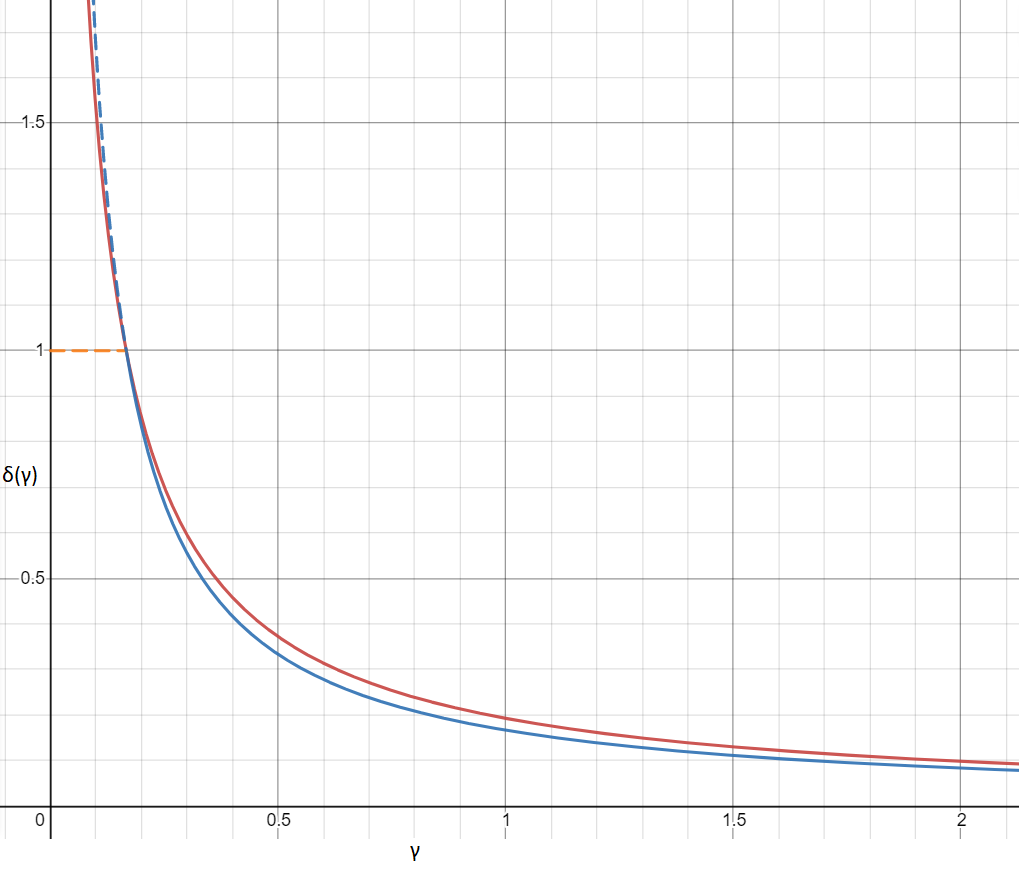
\includegraphics[width=340pt]{\resourceDir/img/Analysis/upper_bound_and_simplified_version.png}
				\end{figure}
				%\clearpage
				
				The red line is the inverse of the function ${ \delta^2 + 5\delta }$ (for positive values) that we have established as an upper bound on the value of ${ \abs{(x^2 + x) - 6} }$ and the blue line is the inverse of $6\delta$ (so ${ \delta = \frac{\epsilon}{6} = \frac{1}{6\gamma} }$).\\
				
				As we can see, for values of ${ \epsilon < 6 \iff \gamma > \frac{1}{6} }$, the blue line is underneath the red line which tells us that if we use those values for $\delta$ then we will definitely satisfy the limit condition. This can be seen more clearly in the below maginification of an area of the graph.\\
				\begin{figure}[h!]
					\centering
					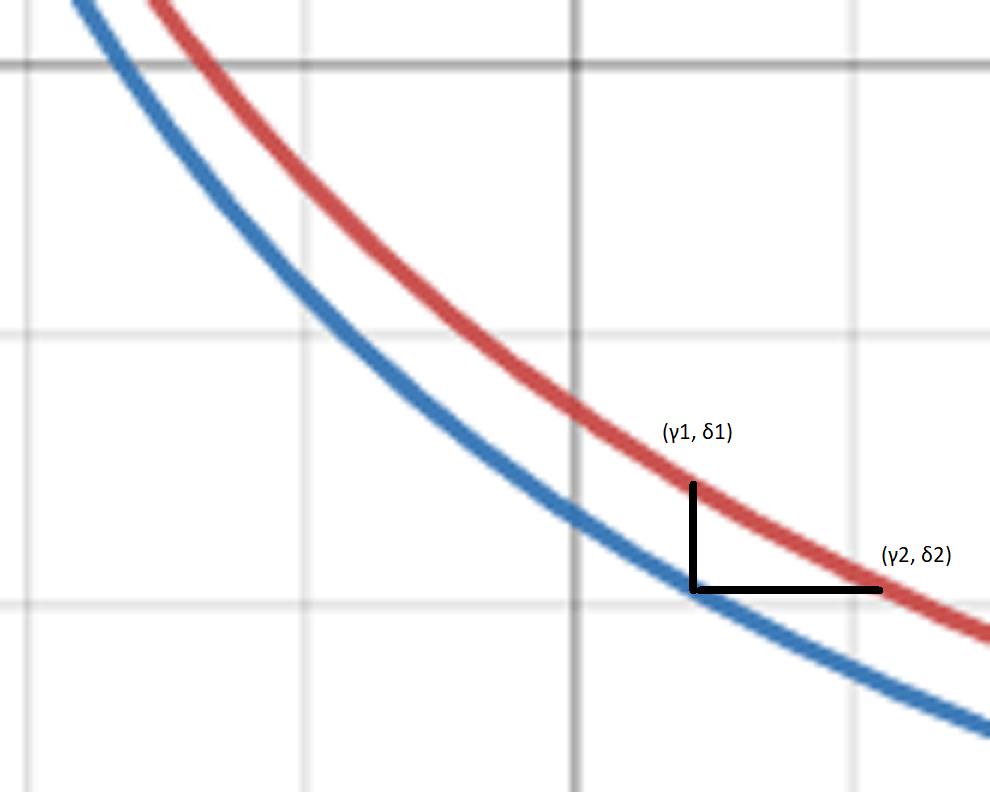
\includegraphics[width=340pt]{\resourceDir/img/Analysis/upper_bound_and_simplified_version_blow_up.png}
				\end{figure}
				
				By using the function represented by the blue line, for the value ${ \gamma = \gamma_1 }$ (which corresponds to some value of $\epsilon$) we return --- instead of $\delta_1$ --- the value $\delta_2$ with ${ \delta_2 < \delta_1 }$. The red line tells us that $\delta_2$ actually suffices for a bound ${ \gamma_2 > \gamma_1 }$. We therefore have
				\[ \abs{x - 2} < \delta_2 \implies \abs{(x^2 + x) - 6} < \frac{1}{\gamma_2} < \frac{1}{\gamma_1} \]
				which shows that the blue line gives a tighter bound than necessary and so is also valid. Referring back to the main graph, we can see that the blue dotted line shows that the blue line crosses the red line at ${ \epsilon = 6 \iff \gamma = \frac{1}{6} }$ and so is no longer valid for achieving the required $\epsilon$-neighbourhood.\\
				
				However, instead, we can use the orange dotted line as values of $\delta$ for the remaining values of $\gamma$. This corresponds to the following function,
				\[\begin{aligned}
					\delta(\epsilon) &= 	\begin{cases}
												\frac{\epsilon}{6} & \epsilon \leq 6 \\
												1 & \epsilon > 6
											\end{cases} \nn
					&= \min \left\{ \frac{\epsilon}{6}, 1 \right\}.
				\end{aligned}\]
			
				If we use this function to define the $\delta$ for any $\epsilon$ then, since \textit{both} 1 and ${ \frac{\epsilon}{6} }$ are an upper bound on the value of $\delta$ (which means that even if $\epsilon$ is arbitrarily large, $\delta$ is still upper-bounded by 1), we can therefore reason that,
				\[ \abs{(x^2 + x) - 6} < \delta (\delta + 5) \leq 6 \delta \leq 6 \frac{\epsilon}{6} = \epsilon. \]
			}
		\end{exe}
	}




% -------------------
\pagebreak
	
	
	
	\subsubsection{Continuity}
	\bigskip
	\boxeddefinition{\textbf{(Continuity at a point)} 
		A function $ f $ is \textit{continuous at a point $a$} if
		\begin{itemize}
			\item{$f(a)$ is defined,}
			\item{${ \lim_{x \to a} f(x) = f(a) }$.}
		\end{itemize}
		\smallskip
		More formally, the definition of ${ \lim_{x \to a} f(x) = L }$ is,
		\[ \forall \epsilon > 0 \logicsep \exists \delta \suchthat 0 < \abs{x - a} < \delta \implies \abs{f(x) - L} < \epsilon. \]
		But if $f(a)$ is defined, then when ${ \abs{x - a} = 0 }$ (i.e. when ${ x = a }$) we have 
		\[ f(x) = f(a) \implies \abs{f(x) - f(a)} = 0 < \epsilon. \]
		Therefore, if $f(a)$ is defined and ${ \lim_{x \to a} f(x) = f(a) }$, then
		\[ \forall \epsilon > 0 \logicsep \exists \delta > 0 \suchthat \abs{x - a} < \delta \implies \abs{f(x) - f(a)} < \epsilon. \]		
	}
	
	\boxeddefinition{\textbf{(Continuous Function)} A function is \textit{continuous} if it is \textit{continuous at every point}.}
	\boxeddefinition{\textbf{(Continuity on a closed interval)} A function is \textit{continuous on the closed interval $[a, b]$} if it is
		\begin{itemize}
			\item{continuous at every point in the open interval ${ (a, b) }$,}
			\item{${ \lim_{x \to a^+} f(x) = f(a) }$,}
			\item{${ \lim_{x \to b^-} f(x) = f(b) }$.}
		\end{itemize}
	}

	\boxeddefinition{\textbf{(Left and Right-Continuity)} A function is \textit{left continuous} or \textit{continuous on the left} at $a$ if,
		\[ \lim_{x \to a-} f(x) = f(a). \]
		Obviously, from the other side, a function can be \textit{right continuous}.
	}

	\labeledProposition{Let ${ f,g : \R{} \to \R{} }$ be functions that are continuous at ${ a \in \R{} }$ and $ c $ be
		any real number. Then ${ \abs{f}, (cf), (f - g), (f + g), (f(x)g(x)) }$ are all continuous at $ a $, and
		${ (f/g)  }$ is continuous provided ${ g(x) \neq 0 }$ for any $ x $ in some neighbourhood of $ a $.}{}
	\begin{proof}
		This follows from the algebra of finite limits of functions given in \autoref{prop:func-finite-limit-algebra}.
	\end{proof}

	\begin{corollary}
		It follows then that every polynomial is continuous. This can be seen as the most simple polynomial is a constant - which is clearly continuous; also ${ f(x) = x }$ is clearly continuous. Then powers of $x$ are continuous as they are products of continuous functions and when multiplied by coefficients this is a constant multiplying a continuous function so the resultant function is continuous. Then any polynomial is a summation of such terms so the result is continuous as the sum of continuous functions is continuous.
	\end{corollary}

	\labeledProposition{If $ g $ is a function which is continuous at $ a $, and $ f $ is a function which is
		continuous at $ g(a) $. Then ${ (f \circ g)  }$ is continuous at $ a $.}{composition-of-continuous-funcs-is-continuous}
	\begin{proof}
		Continuity of $f$ at $g(a)$ guarantees that for any ${ \epsilon > 0 }$ there exists some ${ \delta' > 0 }$ such that ${ \abs{x' - g(a)} < \delta' \implies \abs{f(x') - f(g(a))} < \epsilon }$ and continuity of $g$ at $a$ guarantees that for any ${ \delta' > 0 }$ there exists some ${ \delta > 0 }$ such that ${ \abs{x - a} < \delta \implies \abs{g(x) - g(a)} = \abs{x' - g(a)} < \delta' }$.
	\end{proof}
	\begin{corollary}
		If $ g $ is a function which is continuous at $ a $, and $ f $ is a function which is
		continuous at $ g(a) $. Then,
		\[ \lim_{x \to a} (f \circ g)(x) = \lim_{x \to a} f(g(x)) = f(\lim_{x \to a} g(x)). \]
	\end{corollary}

	\bigskip
	\subsubsection{Functions over sequences}
	The following proposition gives an alternative definition of continuity over convergent sequences rather than explicit subsets of $\R{}$.
	\labeledProposition{A function $ f $ is continuous at $ a $ if and only if for each sequence $ (x_n) $ such that ${ \lim_{n \to \infty} x_n = a  }$ we have ${ \lim_{n \to \infty} f(x_n) = f(a) }$.}{continuity-of-functions-over-sequences}
	\note{
		Before the proof, an important point to note is that this theorem applies to "each sequence" with the described limit. This is important as it is possible to find an individual sequence such that the inference is not valid. For example, the constant sequence ${ \forall n \in \N{} \logicsep x_n = a }$ clearly tends to $a$ as ${ n \to \infty }$ but this would not imply continuity of $f$ as the limit of $f(x_n)$ for such a sequence would amount to saying that ${ f(a) = f(a) }$. The definition of continuity is assertion of the equality of the limit of $f$ over values in the neighbourhood of $a$ (but not at $a$ itself) with the value of $f$ at $a$. So, continuity is implied by the fact that the limit of $f(x_n)$ for the constant sequence $x_n = a$ is equal to the limit of $f(x_n)$ for all other sequences $x_n$ whose limit is $a$.\\
		Another way of looking at it is that $f$ is continuous at $a$ because the limit there equals $f(a)$ however the argument converges to $a$.
	}
	\begin{proof}
		Breaking it down into two propositions we have,
		\begin{equation}
			(\forall x_n \suchthat \lim_{n \to \infty} x_n = a) \; \lim_{n \to \infty} f(x_n) = f(a) \tag{$P_1$}
		\end{equation}
		\begin{equation}
			\forall \epsilon > 0 \logicsep \exists \delta > 0 \logicsep \abs{x - a} < \delta \implies \abs{f(x) - f(a)} < \epsilon \tag{$P_2$}
		\end{equation}
		and we need to show that ${ P_1 \iff P_2. }$\\\\
%			So, to begin with we'll assume $P_1$ and show that ${ P_1 \implies P_2. }$\\
%			Unpacking $P_1$ we have a function $f$ such that
%			\[ \forall \epsilon > 0 \logicsep \exists N \logicsep \forall n > N \in \N{} \logicsep \abs{f(x_n) - f(a)} < \epsilon \tag{1} \] 
%			where $x_n$ is a sequence such that
%			\[ \forall \delta > 0 \logicsep \exists N' \logicsep \forall n > N' \in \N{} \logicsep \abs{x_n - a} < \delta. \tag{2} \]
%			Then, if we choose a particular ${ \epsilon > 0 }$, there exists some $N$ such that for all ${ n > N }$ we have ${ \abs{f(x_n) - f(a)} < \epsilon }$. Now there will also be some $N' \leq N$ so that ${ \forall n > N }$, we also have ${ n > N' }$ and so there is some $\delta$ such that ${ \abs{x_n - a} < \delta }$.\\
%			Furthermore, since $P_1$ says that this is the case \textit{whenever} we have an $x_n$ such as this,
%			\[ \abs{f(x_n) - f(a)} \centernot< \epsilon \implies \abs{x_n - a} \centernot< \delta \]
%			which means that
%			\[ \abs{x_n - a} < \delta \implies \abs{f(x_n) - f(a)} < \epsilon. \]
%			We therefore have,
%			\[ \forall \epsilon > 0 \logicsep \exists \delta > 0 \logicsep \abs{x - a} < \delta \implies \abs{f(x) - f(a)} < \epsilon \]
%			which is the statement of continuity of $f$ in $P_2$. \TODO{is this a valid proof of ${ P_1 \implies P_2 }$?}
		
		
%			Since $P_1$ says that this is the case \textit{whenever} we have an $x_n$ such as this, $P_1$ may be rewritten as
%			\[ \forall \epsilon > 0 \logicsep (\exists N \logicsep \forall n > N \in \N{}) \logicsep \exists \delta > 0 \logicsep \abs{x_n - a} < \delta \implies \abs{f(x_n) - f(a)} < \epsilon. \]
%			\TODO{rewrite this part: show that ${ \forall n > N }$ both bounds are true and that if the bound on the function is not true then the bound on $x_n$ must also not be true -- therefore the implication is proven.}
%			Now, if we remove reference to the number of the term of the sequences - ${ N,n }$ - we have
%			\[ \forall \epsilon > 0 \logicsep \exists \delta > 0 \logicsep \abs{x - a} < \delta \implies \abs{f(x) - f(a)} < \epsilon \]
%			which is the statement of continuity of $f$ in $P_2$.
		
%			\nl[16]
%			Next we prove ${ P_2 \implies P_1. }$\\
%			So now we begin by assuming $P_2$ which was that,
%			\[ \forall \epsilon > 0 \logicsep \exists \delta > 0 \logicsep \abs{x - a} < \delta \implies \abs{f(x) - f(a)} < \epsilon. \]
%			Actually, it is quite easy to apply a similar logic as previously but in reverse to make the converse implication. We can choose any $\epsilon$ and there exists some $\delta$ such that $P_2$ holds. Then, as we have seen previously in (2), $P_1$ tells us that, for this value of $\delta$,
%			\[ \exists N' \logicsep \forall n > N' \in \N{} \logicsep \abs{x_n - a} < \delta \]
%			and $P_2$ tells us that,
%			\[ \abs{x_n - a} < \delta \implies \abs{f(x_n) - f(a)} < \epsilon. \]
%			Putting the two together we get,
%			\[ \forall \epsilon > 0 \logicsep \exists \delta > 0 \logicsep \exists N' \logicsep \forall n > N' \in \N{} \logicsep \abs{x_n - a} < \delta \implies \abs{f(x_n) - f(a)} < \epsilon \]
%			which implies that
%			\[ \forall \epsilon > 0 \logicsep \exists N \logicsep \forall n > N \in \N{} \logicsep \abs{f(x_n) - f(a)} < \epsilon. \]
%			So we have shown that $P_2$ implies that (2) implies (1) which is ${ P_2 \implies P_1 }$ as required.\\\\
		
		
		Unpacking $P_1$ we have a function $f$ such that
		\[ \forall \epsilon > 0 \logicsep \exists N \logicsep \forall n > N \in \N{} \logicsep \abs{f(x_n) - f(a)} < \epsilon \tag{1} \] 
		where $x_n$ is a sequence such that
		\[ \forall \delta > 0 \logicsep \exists N' \logicsep \forall n > N' \in \N{} \logicsep \abs{x_n - a} < \delta. \tag{2} \]
		
		\nl[6]
		Firstly, it is easily shown that ${ P_2 \implies P_1 }$. We begin by assuming $P_2$ which was that,
		\[ \forall \epsilon > 0 \logicsep \exists \delta > 0 \logicsep \abs{x - a} < \delta \implies \abs{f(x) - f(a)} < \epsilon. \]
		We can choose any $\epsilon$ and there exists some $\delta$ such that $P_2$ holds. Then, as we can see in (2), $P_1$ tells us that, for this value of $\delta$,
		\[ \exists N' \logicsep \forall n > N' \in \N{} \logicsep \abs{x_n - a} < \delta \]
		and $P_2$ tells us that,
		\[ \abs{x_n - a} < \delta \implies \abs{f(x_n) - f(a)} < \epsilon. \]
		Putting the two together we get,
		\[ \forall \epsilon > 0 \logicsep \exists \delta > 0 \logicsep \exists N' \logicsep \forall n > N' \in \N{} \logicsep \abs{x_n - a} < \delta \implies \abs{f(x_n) - f(a)} < \epsilon \]
		which implies that
		\[ \forall \epsilon > 0 \logicsep \exists N \logicsep \forall n > N \in \N{} \logicsep \abs{f(x_n) - f(a)} < \epsilon. \]
		So we have shown that $P_2$ implies that (2) implies (1) which is ${ P_2 \implies P_1 }$ as required.\\
		
		\nl[6]
		To prove the converse ${ P_1 \implies P_2 }$ we will use a proof by contradiction.\\
		So, we are assuming $P_1$ but also assuming, for contradiction, that $P_2$ is false. Then we are negating the statement,
		\[ \forall \epsilon > 0 \logicsep \exists \delta > 0 \logicsep \abs{x - a} < \delta \implies \abs{f(x) - f(a)} < \epsilon \]
		so we are asserting that,
		\[ \exists \epsilon > 0 \logicsep \nexists \delta > 0 \logicsep \abs{x - a} < \delta \implies \abs{f(x) - f(a)} < \epsilon \]
		which is equivalent to
		\[ \exists \epsilon > 0 \logicsep \forall \delta > 0 \logicsep \abs{x - a} < \delta \centernot\implies \abs{f(x) - f(a)} < \epsilon \]
		or alternatively,
		\[ \exists \epsilon > 0 \logicsep \forall \delta > 0 \logicsep \exists x \logicsep (\abs{x - a} < \delta) \wedge (\abs{f(x) - f(a)} \geq \epsilon).  \tag{*} \]
		So (*) says that $\lnot{P_2}$ is equivalent to the statement that there exists some ${ \epsilon > 0 }$ such that for all ${ \delta > 0 }$ there will be some $x$ in the $\delta$-neighbourhood of $a$ such that ${ \abs{f(x) - f(a)} \geq \epsilon }$. To prove that this implies $\lnot{P_1}$ we will need to show that it follows that there exists some sequence $x_n$ such that ${ x_n \to a }$ as ${ n \to \infty }$ but also that ${ \lim_{n \to \infty} f(x_n) \neq f(a) }$.\\
		
		Now, if we choose a value of $\delta$ that depends on a natural number $n$ in such a way that ${ \delta \to 0 }$ as ${ n \to \infty }$ -- for example, if ${ \delta = 1/n }$ -- then the $\delta$-neighbourhoods around $a$ will get smaller as ${ n \to \infty. }$ Then we can select an $x$ from the $\delta$-neighbourhood that corresponds to a particular value of $n$ and call it $x_n$ and, in this way, we create a sequence $x_n$ that converges to $a$. So we have ${ \lim_{n \to \infty} x_n = a. }$\\
		
		But now, if we fix the value of $\epsilon$ to a value that satisfies (*) then (*) tells us that, for every $\delta$ there is an $x_n$ in the $\delta$-neighbourhood of $a$ with ${ \abs{f(x_n) - f(a)} \geq \epsilon }$. We can choose this value for $x_n$ and so, construct a sequence $x_n$ that converges to $a$ but
		\[ \lim_{n \to \infty} f(x_n) \neq f(a). \]
		This contradicts hypothesis $P_1$ and so ${ \lnot{P_2} \implies \lnot{P_1} }$.
	\end{proof}
	\begin{corollary}\label{cor:lim_of_func_of_convergent_sequence_is_func_of_limit}
		For a function $f$ that is continuous at $a$, 
		\[ \lim_{n \to \infty} f(x_n) = f\left( \lim_{n \to \infty} x_n \right). \]
	\end{corollary}
	\begin{proof}
		This is just a rewriting of \autoref{prop:continuity-of-functions-over-sequences}.
	\end{proof}

	\biggerskip
	\subsubsection{Continuous Functions on Closed Intervals}
	
	\subsubsection{Examples of continuity}
	\begin{exe}
		\ex{
			The indicator function for rational numbers within the reals, known as the \textbf{Dirichlet Function},
			\[ 
			f(x) =	\begin{cases} 
			0 & x \text{ is irrational} \\
			1 & x \text{ is rational}
			\end{cases}. 
			\]
			This function is nowhere continuous because between every two irrational numbers there is a rational number (and vice-versa) so $f(x)$ is flipping between 0 and 1 in every neighbourhood of every point however small a neighbourhood we consider. So this function never converges anywhere but \textit{is} bounded because it only ever takes values of 1 or 0 so, clearly, its maximum is 1 and minimum is 0.
		}\label{ex:dirichlet_function}
		\bigskip
		\ex{
			The function ${ f(x) = 1/x }$ over the interval ${ (0,1] }$ is continuous at every point but unbounded as it goes to infinity as ${ x \to 0 }$. If we consider the same function over the closed interval ${ [0,1] }$ then we no longer have continuity over this interval as there is a singularity at ${ x = 0 }$.\\
			
			However, if we define the function at ${ x = 0 }$ so that we have a new function,
			\[
				g(x) =
				\begin{cases}
					1/x & x \neq 0 \\
					1 & x = 0
				\end{cases} 
			\]
			then the function $g$ is unbounded on the closed interval ${ [0,1] }$ despite also being defined at every point in the interval. The reason is that we have removed the singularity at 0 by defining a finite value at the point. This creates a jump-discontinuity at 0 so we have sacrificed continuity in order to achieve this.
		}\label{ex:reciprocal_function}
	\end{exe}
	
	\subsubsection{Extreme Value Theorem}
	\TODO{consider rewrite: \\
		If a function $f$ is continous on the closed interval ${ [a,b] }$ then it attains a maximum and minimum on the interval.
	}
	\labeledTheorem{Let $f$ be continous on ${ [a,b] }$. Then $f$ is bounded on ${ [a,b] }$ and it achieves its maximum; that's to say, the supremum is equal to the maximum.}{extreme_value_theorem}
	\note{
		Note that, even if $f$ is defined at every point in ${ [a,b] }$, if it is not continuous then it \textit{may} not be bounded. There \textit{do} exist functions that are not continuous but bounded (for example the Dirichlet Function \ref{ex:dirichlet_function}) but there also exist functions that are not continuous and unbounded such as the reciprocal function \ref{ex:reciprocal_function}. So, functions that are not continuous on a closed interval may be bounded or not; and functions that are continuous on an open interval also may or may not be bounded (again, the reciprocal function is an example of a function that is continuous on an open interval but not bounded); but here we will show that functions that are continuous on a closed interval must be bounded on that interval.
	}
	\begin{proof}
		It may be tempting to begin trying to prove this by reasoning as follows.\\			
		\begin{displayquote}
		That $f$ is continuous on ${ [a,b] }$ means that, for any ${ c \in (a,b) }$,
		\[ \forall \epsilon > 0 \logicsep \exists \delta > 0 \logicsep \abs{x - c} < \delta \implies \abs{f(x) - f(c)} < \epsilon. \]
		This means that the value of $f(x)$ must be finite everywhere in ${ (a,b) }$ as, choosing any fixed point $c$ in the open interval, ${ \abs{x - c} }$ is finite and, therefore, less than some $\delta$ thus implying that ${ \abs{f(x) - f(c)} < \epsilon }$ for some finite $\epsilon \dots$\\
		\end{displayquote}
		
		However this is \textbf{dead wrong!} If we take the example of the reciprocal function (\ref{ex:reciprocal_function}) over the interval ${ (0,1] }$: If we take $x$-values approaching 0, the value of $f(x)$ grows unbounded. For any given $x$-value it will be less than some finite $\epsilon$ but we can always find another $x$-value with a greater value of $f(x)$. So, there is no maximum $\epsilon$ and so, also no maximum value of $f(x)$ on the interval.\\
		
		Another tempting way to prove this is as follows.\\
		
		\begin{displayquote}
		A closed interval is an interval such that every sequence of values in the interval converges to a point in the interval.\\ 
		That $f$ is continuous on ${ [a,b] }$ implies that for every sequence, $x_n$, of values in ${ [a,b] }$ that converges to some point in ${ c \in [a,b] }$, ${ \lim_{n \to \infty} f(x_n) = f(c) }$. Furthermore, that the interval is closed implies that every sequence of values in the interval converges to a point in the interval. Therefore, we can conclude that $f(x)$ at every point in ${ [a,b] }$ exists and is finite so that $f$ is bounded and obtains a maximum on the interval.\\
		\end{displayquote}
		
		There are two issues with this:
		\begin{enumerate}
			\item{The statement about the nature of a closed interval that the proof relies upon has not been proven.}
			\item{That $f(x)$ is defined and finite for all ${ x \in [a,b] }$ is taken as proof that the function is bounded and obtains a maximum in the interval.}
		\end{enumerate}
		To deal with issue (1) -- if we're not going to prove the proposition about closed intervals as a pre-requisite of the proof -- we need to develop a proof that doesn't rely on this characteristic of closed intervals. To deal with (2) meanwhile, we need to explicitly prove boundedness and that $f$ obtains a maximum.\\
		The proof given in LSE Abstract Mathematics course material follows.\\
		
		\begin{displayquote}
		Suppose first that $ f $ is unbounded above. For each ${ n \in N }$, let $ x_n $ be a point in ${ [a, b] }$ such that ${ f(x_n) > n }$. The sequence $ (x_n) $ is bounded, so has a convergent subsequence ${ (x_{k_n}) }$, tending to some limit $ c $ (by Theorem 10.11). Necessarily ${ c \in [a, b] }$. Since $ f $ is continuous at $ c $, ${ f(x_{k_n}) \to f(c) }$ as ${ n \to \infty }$. But this contradicts the construction of the sequence $ (x_n) $, since ${ f(x_{k_n}) > n \to \infty }$. So $ f $ is bounded above. Let ${ M = \text{sup}\setc{f(x)}{x \in [a, b]} }$. For each ${ n \in N }$, let $ x_n $ be a point in ${ [a, b] }$ such that ${ f(x_n) > M - \frac{1}{n} }$. Again take a convergent subsequence ${ (x_{k_n}) }$ of $ (x_n) $, tending to some limit ${ c \in [a, b] }$. Arguing as before, we see ${ f(c) = M }$.
		\end{displayquote}
	
		This proof says: Assume that $f$ is unbounded on the interval. Then we can construct a sequence of $x$-values such that, for the $n$th value $x_n$, ${ f(x_n) > n }$. This is possible because, if $f$ is unbounded, for any value of $n$, there is some subinterval of $x$-values such that for each of them ${ f(x) > n }$ and any interval of the real numbers contains an infinite number of real numbers and so, a sequence $x_n$ with ${ n \to \infty }$. Note that, at this point, $x_n$ is an arbitrary sequence which is not necessarily convergent (it could bounce around the interval).\\
		Then, we notice that this sequence $x_n$ is necessarily bounded (as it is a subinterval of ${ [a,b] }$) and so we invoke the Bolzano-Weierstrass Theorem, \autoref{theo:every_bounded_seq_has_convergent_subseq} (called Theorem 10.11 in the quoted proof), to deduce that it has a convergent subsequence which we call $x_{k_n}$ and call its limit $c$.\\
		At this point we can use the continuity of $f$ on the interval to deduce that ${ f(x_{k_n}) \to f(c) }$ as ${ n \to \infty }$ by which we obtain a contradiction to the condition we set on the values of $x_{k_n}$ when we constructed the sequence -- namely that ${ f(x_{k_n}) > n }$. Notice that this is constructing a sequence $x_{k_n}$ such that $f(x_{k_n})$ grows without bound as ${ n \to \infty }$ and then saying, "but the limit of $x_{k_n}$ as ${ n \to \infty }$ is $c$ which is inside the interval and so (by continuity) the limit of $f(x_{k_n})$ as ${ n \to \infty }$ is $f(c)$ -- a fixed finite value". This is the point where the fact that the interval ${ [a,b] }$ is closed comes into play -- if the interval were not closed it would be possible that $c$ was not inside the interval and then we would not be able to invoke continuity to assert that the limit of $f(x_{k_n})$ over this sequence was finite.\\
		So, now we have shown that if a function is continuous over a closed interval then assuming that the function is unbounded produces a contradiction and, therefore, we can conclude that it is, in fact, bounded.\\
		The last thing that needs to be proven is that $f$ obtains its maximum in the interval. Having shown that the function is bounded on the interval we now know that there exists
		\[ M = \text{sup}\setc{f(x)}{x \in [a, b]} \]
		and we need to show that there is such an $x$-value in ${ [a,b] }$ that ${ f(x) = M }$. In an open interval this might not be the case as the supremum of the function on the interval might occur as the limit of $f$ over a sequence of $x$-values converging to a point that lies outside the interval. So, in this case, we construct a convergent sequence such that ${ f(x_{k_n}) \to M }$ as ${ n \to \infty }$ by selecting $x_n$ such that ${ f(x_n) = M - \frac{1}{n} }$. This is possible because the definition of the supremum says that, because it is the \textit{lowest} upper bound,
		\[ \forall \epsilon > 0 \logicsep \exists f(x_n) \logicsep f(x_n) > M - \epsilon \]
		and so we are letting ${ \epsilon = \frac{1}{n} }$. Then, as previously, we take a convergent subsequence of this sequence and name it $x_{k_n}$. So, as before, we have a sequence converging on some point, we'll call it ${ c \in [a,b] }$, at which $f$ is continuous so that ${ f(x_{k_n}) \to M }$ as ${ n \to \infty }$ implies that ${ M = f(c) }$. This, in turn, means that $f$ obtains a maximum in the interval.			 
	\end{proof}

	\bigskip
	\subsubsection{Intermediate Value Theorem}
	\labeledTheorem{Let $f$ be continuous on ${ [a,b] }$ with ${ f(a) < f(b) }$. Then, for all ${ K \suchthat f(a) < K < f(b) }$, there exists some ${ c \in (a,b) }$ with ${ f(c) = K }$.
	}{intermediate_value_theorem}
	\note{Note that this theorem is \textbf{not} written for an interval such that ${ f(a) \leq f(b) }$ because if ${ f(a) = f(b) }$ then the only ${ K \suchthat f(a) \leq K \leq f(b) }$ is ${ f(a) = K = f(b) }$. But now it is \textbf{not} true to say that there exists some ${ c \in (a,b) }$ with ${ f(c) = K }$ as there is no reason why the value of $f(x)$ at the bounds of the interval should be repeated somewhere in the interior of the interval.}
	\note{\question{What is wrong with the following proof?}
		\begin{proof}Suppose ${ \centernot\exists x \in [a,b] \suchthat f(a) < f(x) < f(b) }$. Since we know that at ${ x = a }$ the value is $f(a)$ and at ${ x = b }$ the value is $f(b)$ with ${ f(b) > f(a) }$, we can deduce that,
		\[ \exists c \in [a,b] \suchthat \lim_{x \to c^-} f(x) = f(a) \land \lim_{x \to c^+} f(x) = f(b). \]
		But this contradicts the hypothesis that $f$ is continuous on the entire interval. Therefore, there must exist some
		\[ x \in [a,b] \suchthat f(a) < f(x) < f(b). \]
		But then we can recursively apply this same logic to the intervals ${ [f(a),f(x)] }$ and ${ [f(x),f(b)] }$ to show that there must be values of $f$ between them also. Since it is always possible for us to apply the reasoning to any interval however small, we can conclude that between any distinct values of the function ${ f(x_1) < f(x_2) }$, there must be an intermediate value of the function ${ f(x_1) < f(x_3) < f(x_2) }$. $\qedhere$	
		\end{proof}
	}
	\medskip
	We begin by proving a special case from which the general proof will follow.
	\begin{lemma}
		Let $f$ be continuous on ${ [a,b] }$ with ${ f(a) < 0 < f(b) }$. Then there exists some ${ c \in (a,b) }$ with ${ f(c) = 0 }$.
	\end{lemma}
	\begin{proof}
		A first attempt at this proof is given below.\\
		\begin{displayquote}
			Continuity at the interval bounds $a$ and $b$ means that, for some ${ \epsilon_1, \epsilon_2 > 0 }$,
			\[ \exists \delta_1 \logicsep 0 \leq x - a < \delta_1 \implies \abs{f(x) - f(a)} < \epsilon_1, \]
			\[ \exists \delta_2 \logicsep 0 \leq b - x < \delta_2 \implies \abs{f(x) - f(b)} < \epsilon_2. \]
			
			So, we have a lower neighbourhood around $f(a)$ and an upper neighbourhood around $f(b)$ as follows,
			\[ f(a) - \epsilon_1 < f(x) < f(a) + \epsilon_1, \]
			\[ f(b) - \epsilon_2 < f(x) < f(b) + \epsilon_2 \]
			If ${ \epsilon_1 > \abs{f(a)} }$ and ${ \epsilon_2 > \abs{f(b)} }$ then both neighbourhoods contain ${ f(x) = 0 }$. Therefore, there is some interval of $x$ such that ${ f(x) }$ lies inside both the lower and upper neighbourhood -- in the overlap of the two. In the overlap we have,
			\[ f(b) - \epsilon_2 < f(x) < f(a) + \epsilon_1. \]
			Now if we let $\epsilon_1$ vary freely but make $\epsilon_2$ a function of $\epsilon_1$ like so,
			\[ \epsilon_2 = f(a) + f(b) + \epsilon_1 \]
			then we still have ${ \epsilon_1 > \abs{f(a)} }$ and ${ \epsilon_2 > \abs{f(b)} }$ as,
			\[ \epsilon_1 > \abs{f(a)} \iff -\epsilon_1 < f(a) < \epsilon_1 \iff 0 < f(a) + \epsilon_1 < 2\epsilon_1 \]
			so ${ \epsilon_2 > f(b) }$ and, conversely, if we assume that ${ \epsilon_2 > \abs{f(b)} }$ then,
			\[ \epsilon_2 > \abs{f(b)} \iff -\epsilon_2 < f(b) < \epsilon_2 \iff -\epsilon_2 - f(b) < 0 < \epsilon_2 - f(b) \]
			\[ \epsilon_1 = \epsilon_2 - f(a) - f(b) > -f(a) = \abs{f(a)} \hspace{20pt}\sidecomment{since ${ f(a) < 0 }$}. \]
			Therefore,
			\[ \epsilon_2 = f(a) + f(b) + \epsilon_1 \implies [ \epsilon_1 > \abs{f(a)} \iff \epsilon_2 > \abs{f(b)} ]. \]
			Now we have,
			\[ f(b) - \epsilon_2 = -f(a) - \epsilon_1 < f(x) < f(a) + \epsilon_1 \]
			which is equivalent to
			\[ \abs{f(x)} < f(a) + \epsilon_1 = \epsilon_3. \]
			Now, since ${ f(a) + \epsilon_1 > 0 }$ we also have ${ \epsilon_3 > 0 }$ and it can become arbitrarily small by making ${ \abs{f(a)} - \epsilon_1 }$ arbitrarily small. So we have shown that continuity over the closed interval and ${ f(a) < f(b) }$ imply that we can find subintervals of ${ [a,b] }$ such that ${ f(x) }$ is constricted to ever-decreasing neighbourhoods of 0. In other words, for some ${c \suchthat a < c < b, \; f(x) \to 0 }$ as  ${ x \to c }$ and since $f$ is continuous on the interval this implies that ${ f(c) = 0 }$ also. 
		\end{displayquote}
		This is not bad but suffers from vagueness in a couple of areas: the overlap of the lower and upper neighbourhoods probably needs to be more precisely defined and, certainly, the final part of the proof stating that confining $f(x)$ to ever-decreasing neighbourhoods of 0 implies that there is some $c$ such that ${ f(c) = 0 }$ needs to be drawn much more explicitly.\\\\
		Here is the proof given in LSE Abstract Mathematics.\\
		\begin{displayquote}
			We construct a sequence of intervals ${ [a_n, b_n] }$ such that
			\begin{enumerate}
				\item{${ f(a_n) < 0,\; f(b_n) > 0 }$ for each $ n $}
				\item{${ [a_{n+1}, b_{n+1}] \subseteq [a_n, b_n] }$ for each $ n $.}
			\end{enumerate}				
			We start by letting ${ [a_1, b_1] = [a, b]. }$ Then for each ${ n \geq 1 }$, we define ${ [a_{n+1}, b_{n+1}] }$ as follows.\\
			
			Let ${ c_n = (a_n + b_n)/2 }$, be the midpoint of the previous interval. If ${ f(c_n) = 0, }$ then the
			theorem is proved and so we need not continue constructing intervals!\\
			
			Otherwise, if ${ f(c_n) < 0 }$, we define ${ a_{n+1} = c_n }$ and ${ b_{n+1} = b_n }$. And if ${ f(c_n) > 0 }$, we define
			${ b_{n+1} = c_n }$ and ${ a_{n+1} = a_n }$. Note that the condition 1. is satisfied by choosing our intervals in this manner.
			Moreover, note that the ${ (n + 1) }$st interval is half the size of the $n$th interval and so
			${ b_{n+1} - a_{n+1} \leq (b_1 - a_1)/2^n }$. It follows that
			\[ \lim_{n \to \infty} (b_n - a_n) = 0.  \tag{3}\]
			
			Finally, note that $ (a_n) $ is increasing and bounded above (by $ b_1 $) and so it has a limit; similarly $ (b_n) $ is decreasing and bounded below and so has a limit. Thus by (3) (and algebra of limits) these limits are equal to, say, c. Thus by continuity (using \autoref{prop:continuity-of-functions-over-sequences}),
			\[ f(c) = \lim_{n \to \infty} f(b_n) \geq 0, \]
			where the last inequality follows from the fact that each ${ f(b_n) \geq 0 }$ (in fact > 0). Similarly,
			\[ f(c) = \lim_{n \to \infty} f(a_n) \leq 0. \]
			Thus $ f(c) $ must be equal to zero, and the proof is complete.
		\end{displayquote}
	\end{proof}
	Clearly, the general proof of the Intermediate Value Theorem follows naturally from this because,
	\begin{itemize}
		\item{If ${ f(a) > f(b) }$ then we can consider the function ${ g(x) = -f(x) }$ so that we have ${ g(a) < g(b) }$,}
		\item{If we have ${ K \suchthat f(a) < K < f(b) }$ with ${ K \neq 0 }$ we can consider ${ g(x) = f(x) - K }$ so that we have ${ g(a) < 0 < g(b) }$.}
	\end{itemize}
	So, the general problem posed in the Intermediate Value Theorem is reducible to the case we have proved.
	
	\bigskip
	\begin{corollary}
		\label{coro:continuous_func_mapping_interval_to_itself_has_invariant_point}
		Suppose that the real function $f$ is continuous on the closed interval ${ [a,b] }$ and that $f$ maps ${ [a,b] }$ into ${ [a,b] }$. Then there is ${ c \in [a,b] }$ with ${ f(c) = c }$.
	\end{corollary}
	\begin{proof}
		Let ${ h(x) = f(x) - x }$ so that ${ f(c) = c }$ if and only if ${ h(c) = 0 }$. Then also we have,
		\[ a \leq f(x) \leq b \implies h(a) \geq 0,\; h(b) \leq 0. \]
		But this means that, either one of $h(a)$ or $h(b)$ is equal to 0 or neither are. In the case that one of them is equal to 0 then we have found our $c$ such that ${ f(c) = c }$. Otherwise, if neither is equal to 0, then we must have ${ h(a) > 0 }$ and ${ h(b) < 0 }$. So, we may apply the Intermediate Value Theorem to conclude that there exists ${ c \in (a,b) }$ such that ${ h(c) = 0 }$ which is to say ${ f(c) = c }$.
	\end{proof}

	\bigskip
	\subsubsection{Examples of reasoning with the Intermediate Value Theorem}
	\begin{exe}
		\ex{\textit{Suppose the real function $f$ is continuous, positive and unbounded on $\R{}$ and that ${ \inf \setc{f(x)}{x \in \R{}} = 0 }$. Use the Intermediate Value Theorem to prove that the range of $f$ is ${ (0,\infty) }$. }\\\\
			Let ${ y \in (0,1) }$. We show that there is some ${ c \in \R{} }$ such that ${ f(c) = y }$. This shows that the range is the whole of ${ (0,1) }$. (The fact that it is no larger follows from the given fact that $ f $ is positive.)\\
			Now,  ${ \text{inf}\,f(\R{}) = \text{inf}\,\setc{f(x)}{x \in \R{}} = 0 }$, so, since ${ y > 0 }$, there must be some ${ y_1 \in f(\R{}) }$ with ${ y_1 < y }$. This means there is some ${ x_1 \in \R{} }$ such that ${ y_1 = f(x_1) < y }$.\\
			Similarly, because $ f $ is unbounded, which means $ f(\R{}) $ is unbounded, there must be some ${ y_2 \in f(\R{}) }$ with ${ y_2 > y }$ and there will be some ${ x_2 \in \R{} }$ such that ${ y_2 = f(x_2) > y }$.\\
			Then $ y $ lies between $ f(x_1) $ and $ f(x_2) $ and, since $ f $ is continuous, the Intermediate Value Theorem shows that there is some $ c $ between $ x_1 $ and $ x_2 $ with ${ f(c) = y }$.
		}
			\ex{\textit{Suppose the real function $g$ is continuous on $\R{}$ and that $g$ maps ${ [a,b] }$ into ${ [d,e] }$ and maps ${ [d,e] }$ into ${ [a,b] }$ where ${ a < b,\; d < e }$. By considering the function
					\[ k(x) = g(g(x)), \]
			prove that there are ${ p,q \in \R{} }$ such that
				\[ g(p) = q,\; g(q) = p. \]
			Hence show that there is ${ c \in \R{} }$ such that ${ g(c) = c }$.
			}\\\\
			The function $k$, being a composition of continuous functions, is continuous and also maps ${ [a,b] }$ into ${ [a,b] }$ so that we can use \autoref{coro:continuous_func_mapping_interval_to_itself_has_invariant_point} to deduce that there exists ${ c \in [a,b] }$ such that ${ k(c) = c }$. If we let ${ p = c }$ and ${ q = g(p) }$ then we have,
			\[ k(p) = p \iff g(g(p)) = p \iff g(q) = p. \]
			Now we can employ the same trick again by defining
			\[ h(x) = g(x) - x \]
			and then we have
			\[ h(p) = g(p) - p = q - p, \; h(q) = g(q) - q = p - q \]
			so that ${ h(p) = -h(q) }$ and, therefore, ${ h(x) }$ changes sign between $p$ and $q$. (Note that we don't know which of $p$ and $q$ is the lower end and upper end of the interval but we know that between the two values the function changes sign.) Then, applying the Intermediate Value Theorem we have some $c$ between $p$ and $q$ such that,
			\[ h(c) = 0 \iff g(c) - c = 0 \iff g(c) = c. \]
		}
	\end{exe}
	





% ----------- break ------------
\pagebreak
	
	
	
	\subsubsection{Relationship Between Sequences and Functions}\bigskip
	Let ${ f: \R{} \mapsto \R{},\; f(x) = y. }$ Now imagine that we take regular intervals on the domain, say, interval 1. We name the $x$-values at the upper bound of these intervals $x_1, x_2, \dots$ for $x = 1, 2, \dots$. Then, the corresponding $y$-values, $y = f(x_1), f(x_2), \dots$ can be named $y_1, y_2, \dots$. In this way, we have defined a sequence, ${ y_n = f(x_n) }$ where ${ x_n \in \N{} }$ (note that this is a different notation from that used before where a sequence ${ x_n = f(n) }$ for ${ n \in \N{} }$).\\
	Looking at the derivative of the function,
	\[ \frac{dy}{dx} \approxeq \frac{\Delta y}{\Delta x} = \frac{ f(x_{n+1}) - f(x_n) }{1} = f(x_{n+1}) - f(x_n). \]
	While the ratio of consecutive terms is,
	\[ \frac{y_{n+1}}{y_n} = \frac{y_n + \Delta y}{y_n} = \frac{f(x_{n+1})}{f(x_n)} =  \frac{f(x_n) + (f(x_{n+1}) - f(x_n))}{f(x_n)}. \]
	Note, also, that
	\[ \frac{y_n + \Delta y}{y_n} = 1 + \frac{\Delta y}{y_n} \approxeq 1 + \frac{dy/dx}{y} = 1 + \frac{d}{dx} \ln{y} \]
	which is to say that ${ \frac{\Delta y}{y_n} }$ is the discrete form of the log derivative.
	Clearly, when ${ \Delta y > 0 }$, we can put this in the form
	\[ \frac{y_{n+1}}{y_n} = 1 + \frac{\Delta y}{y_n} = 1 + \frac{ \Delta y/y_n }{1} = \frac{1 + h}{1}. \]
	If ${ \Delta y < 0 }$ however,
	\[ \frac{y_n + \Delta y}{y_n} = \frac{1}{y_n/(y_n + \Delta y)} = \frac{1}{\frac{y_n + \Delta y - \Delta y}{y_n + \Delta y}} = \frac{1}{1 + \frac{-\Delta y}{y_n + \Delta y}} = \frac{1}{1 + h}. \]
	If ${ \frac{\Delta y}{y_n} }$ does not go to 0 then the ratio of consecutive terms stays below 1 and the sequence converges to 0. If it does go to 0 then the ratio of consecutive terms goes to 1 and the sequence may converge to 0 or to some non-zero value. These cases appear (proof?) to be distinguishable by looking at how fast ${ \frac{\Delta y}{y_n} }$ goes to 0. For example,
	\begin{enumerate}[label=(\roman*)]
		
		\item{${\bm{ a_n = \frac{1}{n} + 1 }}$}
		\[ \lim_{n \to \infty} \frac{1}{n} + 1 = 1 \]
		\[ \frac{\Delta a}{a_n} = \frac{-1}{(n+1)^2} \]
		
		\item{${\bm{ a_n = \frac{1}{n} }}$}
		\[ \lim_{n \to \infty} \frac{1}{n} = 0 \]
		\[ \frac{\Delta a}{a_n} = \frac{-1}{n+1} \]
	\end{enumerate}
	Maybe the fact that ${ \frac{\Delta y}{y_n} }$ goes to 0 faster as ${ n \to \infty }$ in the first case indicates that it converges before it gets to 0?




% -------------- break ----------------
\pagebreak


	\searchableSubsection{Series}{analysis, real analysis}{
		\bigskip
	}



% -------------- break ----------------
\pagebreak


	\searchableSubsection{Differentiation}{analysis, real analysis}{
		\bigskip
	}
  
\end{document}